\fenicschapter{A comparison of some finite element schemes for the incompressible Navier--Stokes equations}
              {A comparison of some finite element schemes for the incompressible Navier--Stokes equations}
              {K. Valen-Sendstad, A. Logg, K.-A. Mardal, H. Narayanan and M. Mortensen}
              {kvs-1}

\newcommand{\css}[1]{$\mathrm{CSS}_{#1}$}

\newcommand{\scheme}[3]{%
\begin{figure*}
  \begin{center}
    \small
    \begin{tabular}{l}
      \hline
      \textbf{Scheme #1:} #2 \\
      \hline
      \begin{minipage}{0.9\textwidth}
        \vspace{0.1cm}
        \begin{enumerate}
          #3
        \end{enumerate}
        \vspace{0.1cm}
      \end{minipage} \\
      \hline
    \end{tabular}
    \normalsize
  \end{center}
\end{figure*}}

Numerical algorithms for the computation of fluid flow have been
an active area of research for several decades and still remains an
active area of research. As a result, there exists a large literature
on discretization schemes for the incompressible Navier--Stokes
equations, and it can be hard to judge which method works best for any
particular problem. Furthermore, since the development of any particular
discretization scheme is often a long process and tied to a specific
implementation, comparisons of different methods are seldom made.

FEniCS is a flexible platform for the implementation of different
kinds of schemes based on finite element methods. To illustrate the
simplicity by which different schemes can be implemented in FEniCS,
we have implemented a test consisting of six different schemes. All
schemes have been tested on six different test problems to compare
the schemes in terms of their accuracy and efficiency. The schemes we
have implemented are Chorin's projection scheme by \citet{Chorin1968}
and \citet{Temam1969}, the incremental pressure correction scheme
(IPCS) by \citet{Goda1979}, the consistent splitting scheme (CSS)
by \citet{GuermondMinevShen2006}, a least-squares stabilized Galerkin
scheme (G2) by \citet{HoffmanJohnson2007}, and a saddle-point solver
based on a Richardson iteration on the pressure Schur complement (GRPC)
as described in \citet{Turek1996}.

All solvers and test problems have been implemented in Python (with a
few C++ extensions) using DOLFIN. The source code for all solvers and
 test problems is available
online\footnote{\url{http://launchpad.net/nsbench/}} and can be used to
reproduce all results shown in this chapter.

%------------------------------------------------------------------------------
\section{Preliminaries}

We consider the incompressible Navier--Stokes equations with unit
fluid density written in the form
\begin{align}
  \label{eq:ns,mom}
  \dot{u} + \nabla u \, u - \nabla \cdot \sigma  &= f, \\
  \label{eq:ns,con}
  \nabla \cdot u &= 0,
\end{align}
where $\sigma$ is the Cauchy stress tensor which for a Newtonian fluid
is defined as
\begin{equation}
  \sigma(u,p) = 2\nu\varepsilon(u) - pI.
\end{equation}
Here, $u$ is the unknown velocity vector, $p$ is the unknown pressure,
$\nu$ is the (kinematic) viscosity, $f$ is the body force per unit
volume, and $\epsilon(u)$ is the symmetric gradient:
\begin{equation}
  \epsilon(u) = \frac{1}{2} (\nabla u + \nabla u^{\top}).
\end{equation}
The above quantities $\sigma$ and $\epsilon$ may be defined as follows
in DOLFIN/UFL:
\begin{python}
def epsilon(u):
    return 0.5*(grad(u) + grad(u).T)
\end{python}
\begin{python}
def sigma(u, p, nu):
    return 2*nu*epsilon(u) - p*Identity(u.cell().d)
\end{python}

In all discretization schemes below, $V_h$ and $Q_h$ refer to the
discrete finite element spaces used to discretize the velocity~$u$ and
pressure $p$, respectively. For all schemes except the G2 scheme,
$V_h$ is the space of vector-valued continuous piecewise quadratic
polynomials, and $Q_h$ is the space of scalar continuous piecewise
linear polynomials (Taylor--Hood elements). For the G2 scheme,
continuous piecewise linears are used for both the velocity and the
pressure. We will further use~$h$ to denote the local mesh size, $k_n
= t_n - t_{n-1}$ to denote the size of the local time step, and $D^n_t
u_h$ to denote the discretized form of the time derivative $(u_h^n -
u_h^{n-1})/k_n$. For all schemes, except the fully implicit schemes G2
and GRPC described below, the convective term is treated explicitly.

%------------------------------------------------------------------------------
\section{Implementation}

We have implemented the solvers and test problems as two
class-hierarchies in Python, where the base classes are \emp{SolverBase}
and \emp{ProblemBase}, respectively.  The solvers, derived from
\emp{SolverBase} implement the scheme, that is, they define the
finite element spaces, assemble and solve linear systems, and perform
time-stepping. Code from several solvers will be shown throughout this
chapter. The problems, derived from the \emp{ProblemBase} class, define
the mesh, initial and boundary conditions, and other parameters.

A main script~\emp{ns} allows a user to solve a given problem with a
given solver. All available problems and solvers may be listed by typing
\begin{bash}
$ ns list
\end{bash}
which results in the following output:
\begin{bash}
Usage: ns problem solver

Available problems:

  drivencavity
  channel
  taylorgreen
  cylinder
  beltrami
  aneurysm

Available solvers:

  chorin
  css1
  css2
  ipcs
  g2
  grpc
\end{bash}

The \emp{ns} script accepts a number of optional parameters to enable
refinement in space and time, storing the solution in VTK or DOLFIN
XML format, computing stresses, or plotting the solution directly to
screen. As an example, to solve the lid-driven cavity test problem
using Chorin's method and plot the solution, one may issue the
following command:
\begin{bash}
$ ns drivencavity chorin plot_solution=True
\end{bash}
Another script named \emp{bench} allows a user to iterate over all
solvers for a given problem, over all problems for a given solver, or
over all problems and all solvers. As an example, the following command
may be used to solve the channel test problem with all solvers on a mesh
refined twice:
\begin{bash}
$ bench channel refinement_level=2
\end{bash}

%------------------------------------------------------------------------------
\section{Solvers}
\label{methods}

In this section, we present an overview of the six different schemes
that have been tested.

\subsection{Chorin's projection method}
\label{sec:chorin}

This scheme, often referred to as a non-incremental pressure
correction scheme was first proposed by \citet{Chorin1968}
and \citet{Temam1969}. For simplicity, we will here refer to this
scheme as \emph{Chorin}. To solve the system of
equations~\eqref{eq:ns,mom}--\eqref{eq:ns,con}, the idea is to first
compute a tentative velocity by neglecting the pressure in the
momentum equation and then projecting the velocity onto the space of
divergence free vector fields. The projection step is a Darcy problem
for $u_h^n$ and $p^n_h$:
\begin{align}
  \frac{u_h^n -u_h^{\bigstar}}{k_n} + \nabla p^n_h &= 0, \\
 \nabla \cdot u_h^n &= 0,
\end{align}
which is in fact reducible to a Poisson problem $-\Delta p^n_h =
- \nabla \cdot u_h^{\bigstar} / k_n$ for the corrected pressure
$p^n_h$. This is summarized in Scheme~1 and the implementation is
shown in Figure~\ref{fig:chorin_code}.  We note that since the
velocity correction step is implemented as the solution of a linear
system (involving a mass matrix that has not been lumped), the
discrete incompressibility constraint is not satisfied exactly. On the
other hand, the Dirichlet boundary conditions for the velocity are
applied strongly as part of the velocity correction step and are thus
satisfied exactly (at the nodal points).

\scheme{1}{Chorin's projection method}
{
\item
  Compute a tentative velocity $u_h^\bigstar$ by solving
  \begin{equation}\label{eq:chorin,1}
    \renni{v}{D_t^n u_h^\bigstar}
    + \renni{v}{\nabla u_h^{n-1} \, u_h^{n-1}}
    + \renni{\nabla v}{\nu \nabla u_h^{\bigstar}}
    = \renni{v}{f^n} \quad \foralls v \in V_h,
  \end{equation}
  including any boundary conditions for the velocity.

\item
  Compute the corrected pressure $p_h^n$ by solving
  \begin{equation}\label{eq:chorin,2}
    \renni{\nabla q}{\nabla p_h^n}
    = -\renni{q}{\nabla \cdot u_h^{\bigstar}} / k_n \quad \foralls q \in Q_h,
  \end{equation}
  including any boundary conditions for the pressure.

\item
  Compute the corrected velocity $u_h^n$ by solving
  \begin{equation}\label{eq:chorin,3}
    \renni{v}{u_h^n} = \renni{v}{u_h^{\bigstar}} - k_n \renni{v}{\nabla p_h^n}
    \quad \foralls v \in V_h,
  \end{equation}
  including any boundary conditions for the velocity.
}

\begin{figure}
  \begin{center}
    \begin{python}
# Tentative velocity step
F1 = (1/k)*inner(u - u0, v)*dx \
   + inner(grad(u0)*u0, v)*dx \
   + nu*inner(grad(u), grad(v))*dx - inner(f, v)*dx
a1 = lhs(F1)
L1 = rhs(F1)

# Poisson problem for the pressure
a2 = inner(grad(p), grad(q))*dx
L2 = -(1/k)*div(us)*q*dx

# Velocity update
a3 = inner(u, v)*dx
L3 = inner(us, v)*dx - k*inner(grad(p1), v)*dx
    \end{python}
    \caption{Implementation of variational forms for the Chorin solver.}
    \label{fig:chorin_code}
  \end{center}
\end{figure}

\subsection{Incremental pressure correction scheme (IPCS)}
\label{sec:ipcs}

An improvement of the non-incremental pressure correction scheme is
possible if the previous value for the pressure is used to compute the
tentative velocity. This idea was first introduced
by \citet{Goda1979}. The IPCS scheme is summarized in Scheme~2 and the
implementation is shown in Figure~\ref{fig:IPCS}. The IPCS scheme as
implemented here also differs from the Chorin scheme in that the
viscous term is evaluated at $(t_{n-1} + t_n)/2$ and a stress
formulation is used in place of the Laplacian formulation used for the
Chorin scheme. Note the importance of the term $\renni{v}{\nu
(\nabla u_h^{n-1/2})^{\top} n}_{\partial\Omega}$ which arises
as a result of integrating the stress term by parts. Without this
term, an incorrect velocity profile is obtained at inlets and outlets
where the velocity will tend to ``creep'' around the corners.

\scheme{2}{Incremental pressure correction (IPCS)}
{
\item
  Compute the tentative velocity $u_h^\bigstar$ by solving
  \begin{multline}\label{eq:ipcs,1}
      \renni{v}{D_t^n u_h^{\bigstar}}
      + \renni{v}{\nabla u_h^{n-1} \, u_h^{n-1}}
      + \renni{\epsilon(v)}{\sigma(u_h^{n-\frac{1}{2}}, p^{n-1}_h)}
      + \renni{v}{p^{n-1}_h n}_{\partial\Omega}
      \\
      - \renni{v}{\nu (\nabla u_h^{n-\frac{1}{2}})^{\top} n}_{\partial\Omega}
      = \renni{v}{f^n}
  \end{multline}
  for all $v \in V_h$, including any boundary conditions for the
  velocity. Here, $u_h^{n-\frac{1}{2}} = (u_h^{\bigstar} + u_h^{n-1}) / 2$.

\item
  Compute the corrected pressure $p_h^n$ by solving
  \begin{equation}\label{eq:ipcs,2}
    \renni{\nabla q}{\nabla p^n_h}
    = \renni{\nabla q}{\nabla p^{n-1}_h} - \renni{q}{\nabla \cdot u_h^{\bigstar}} / k_n,
  \end{equation}
  including any boundary conditions for the pressure.

\item
  Compute the corrected velocity $u_h^n$ by solving
  \begin{equation}\label{eq:ipcs,3}
    \renni{v}{u_h^n} = \renni{v}{u_h^{\bigstar}} - k_n\renni{v}{\nabla(p_h^n-p_h^{n-1})}
    \quad \foralls v \in V_h,
  \end{equation}
  including any boundary conditions for the
  velocity.
  \label{ipcs_listing}
}

\begin{figure}
  \begin{center}
    \begin{python}
# Tentative velocity step
U = 0.5*(u0 + u)
F1 = (1/k)*inner(u - u0, v)*dx \
   + inner(grad(u0)*u0, v)*dx \
   + inner(sigma(U, p0, nu), epsilon(v))*dx \
   + inner(p0*n, v)*ds \
   - beta*nu*inner(grad(U).T*n, v)*ds \
   - inner(f, v)*dx
a1 = lhs(F1)
L1 = rhs(F1)

# Pressure correction
a2 = inner(grad(p), grad(q))*dx
L2 = inner(grad(p0), grad(q))*dx \
   - (1.0/k)*div(u1)*q*dx

# Velocity correction
a3 = inner(u, v)*dx
L3 = inner(u1, v)*dx - k*inner(grad(p1 - p0), v)*dx
    \end{python}
    \caption{Implementation of variational forms for the IPCS
      solver. The flag \emp{beta = 1} is set to zero in the case when
      periodic boundary conditions are used.}
    \label{fig:IPCS}
  \end{center}
\end{figure}

\subsection{Consistent splitting scheme (CSS)}
\label{sec:css}

The consistent splitting scheme, as described
in \citet{GuermondMinevShen2006,GuermondShen2003}, is derived
differently from the other splitting schemes and requires a more
detailed description. The scheme is based on deriving an equation for
the pressure~$p$ by testing the momentum equation~\eqref{eq:ns,mom}
against $\nabla q$.  In combination with the incompressibility
constraint, an equation for the pressure results. After solving for
the pressure, the velocity is updated based solely on the momentum
equation by an appropriate approximation (extrapolation) of the
pressure. The derivation of the consistent splitting scheme is as
follows. Multiply the momentum equation~\eqref{eq:ns,mom} by $\nabla
q$ for $q
\in H^1(\Omega)$ and integrate over the domain~$\Omega$ to obtain
$\renni{\nabla q}{\dot{u} + \nabla u \, u - \nu \Delta u + \nabla
  p} = \renni{\nabla q}{f}$. Since $\renni{\nabla q}{\dot{u}} =
\renni{-q}{\nabla \cdot \dot{u}} + \renni{qn}{\dot{u}}_{\partial
  \Omega}$, it follows by~(\ref{eq:ns,con}) that
\begin{equation}\label{eq:css,laplace}
  \renni{\nabla q}{\nabla p} = \renni{\nabla q}{f - \nabla u \, u +
    \nu \Delta u},
\end{equation}
if we assume that $\dot{u} = 0$ on~$\partial\Omega$. Next, we use the
identity $\Delta v \equiv \nabla \nabla \cdot v - \nabla \times \nabla
\times v$ together with the incompressibility
constraint~(\ref{eq:ns,con}) to write the diffusive term
of~(\ref{eq:css,laplace}) in
\emph{rotational form}:
\begin{equation}\label{eq:css,curl}
  \renni{\nabla q}{\nabla p} = \renni{\nabla q}{f - \nabla u \, u -
    \nu \nabla \times \nabla \times u}.
\end{equation}
This equation is the basis for the consistent splitting scheme. At
this point, we may formulate the CSS scheme as the solution of the
following pair of variational problems:
\begin{equation} \label{eq:css,u}
  \inner{D_t^n u_h}{v}
  + \inner{\nabla u_h^{n-1} \, u_h^{n-1}}{v}
  + \inner{\nu \nabla u_h^n}{\nabla v}
  - \inner{p_h^{\bigstar}}{\nabla \cdot v}
  = \inner{f^n}{v},
\end{equation}
\begin{equation} \label{eq:css,pn}
  \renni{\nabla q}{\nabla p_h^n} =
  \renni{\nabla q}{f^n -\nabla u_h^{n-1} \, u_h^{n-1} - \nu \nabla \times \nabla \times u_h^n},
\end{equation}
where $D_t^n u_h$ is an appropriate approximation of $\dot{u}_h$ and
$p^{\bigstar}_h$ is an appropriate approximation of the pressure. In
the simplest case, one may chose $p_h^{\bigstar} = p_h^{n-1}$ but
higher order approximations are also possible. For example, one may
take $p_h^{\bigstar}$ to be the linear extrapolation of $p_h$ from
$p_h^{n-2}$ and $p_h^{n-1}$ given by $p_h^{\bigstar} = p_h^{n-1} +
(p_h^{n-1} - p_h^{n-2}) = 2p_h^{n-1} - p_h^{n-2}$. We will refer to
the simplest approximation as \css{1} and to the higher-order
approximation as \css{2}.

To avoid having to compute the term~$\nabla \times \nabla \times
u_h^n$ in~(\ref{eq:css,pn}), we take the inner product
of~(\ref{eq:css,u}) with~$\nabla q$ and subtract the result
from~(\ref{eq:css,pn}) to obtain
\begin{equation}\label{eq:css,tmp}
 \begin{split}
   \renni{\nabla q}{\nabla p_h^n - \nabla p_h^{\bigstar}}
   &=
   \renni{\nabla q}{D_t^n u_h
   - \nu \nabla \times \nabla \times u_h^n - \nu \Delta u_h^n} \\
   &=
   \renni{\nabla q}{D_t^n u_h - \nu \nabla \nabla \cdot u_h^n},
 \end{split}
\end{equation}
where we have again used the identity $\Delta v \equiv \nabla \nabla
\cdot v - \nabla \times \nabla \times v$. Finally, we define an
auxiliary field $\psi_h^n = p_h^n - p_h^{\bigstar} + \nu \nabla
\cdot u_h^n$ to write~(\ref{eq:css,tmp}) in the form
\begin{equation}
  \renni{\nabla q}{\nabla \psi_h^n}
  = \renni{\nabla q}{D_t^n u_h}.
\end{equation}
The CSS scheme is summarized in Scheme~3/4.

\scheme{3/4}{Consistent splitting}
{
\item
  Compute the pressure approximation (extrapolation)
  $p_h^{\bigstar}$ by
  \begin{equation}\label{eq:css,1a}
    p_h^{\bigstar} =
    \left\{
    \begin{array}{ll}
      p_h^{n-1}, & \mbox{ for } \mathrm{CSS}_1, \\
      2 p_h^{n-1} - p_h^{n-2}, & \mbox{ for } \mathrm{CSS}_2.
    \end{array}
    \right.
  \end{equation}

\item
  Compute the velocity $u_h^n$ by solving
  \begin{equation}\label{eq:css,2}
    \begin{split}
      \renni{v}{D_t^n u_h}
      + \renni{v}{\nabla u_h^{n-1} \, u_h^{n-1}}
      + \renni{\epsilon(v)}{\sigma(u^{n-\frac{1}{2}}_h, p_h^{\bigstar})}
      + \renni{v}{\bar{p} n}_{\partial\Omega}
      - \renni{v}{\nu (\nabla \bar{u}_h^n)^{\top} n}_{\partial\Omega}
      = \renni{v}{f^n},
    \end{split}
  \end{equation}
  including any boundary conditions for the velocity. Here,
  $u^{n-\frac{1}{2}}_h = (u_h^n + u_h^{n-1}) / 2$ and $\bar{p}$ is a given
  boundary condition for the pressure.

\item
  Compute the pressure correction $\psi_h^n$ by solving
  \begin{equation}\label{eq:css,3}
    \renni{\nabla q}{\nabla \psi_h^n}
    = \renni{\nabla q}{u_h^n - u_h^{n-1}} / k_n
    - \renni{qn}{u_h^n - u_h^{n-1}}_{\partial\Omega} / k_n
    \quad \foralls q \in Q_h.
  \end{equation}

\item
  Compute the corrected pressure $p_h^n$ by solving
  \begin{equation}\label{eq:css,4}
    \renni{q}{p_h^n} = \renni{q}{p_h^{\bigstar} + \psi_h^n - \nu \nabla \cdot u_h^n}
    \quad \foralls q \in Q_h,
  \end{equation}
  including any boundary conditions for the pressure.
}

To solve for the auxiliary variable $\psi$, appropriate boundary
conditions must be used. Since $\psi$ is a \emph{pressure correction}
and not the pressure itself, we use homogenized versions of the
pressure boundary conditions which are zero at the boundary in the
case of Dirichlet boundary conditions. This can be accomplished in
DOLFIN using the function \emp{homogenize}.

We remark that the derivation of the consistent splitting scheme is
based on the assumption that $\dot{u} = 0$ on~$\partial\Omega$ which
gives $\renni{\nabla q}{\dot{u}} = -\renni{q}{\nabla \cdot u} +
\renni{qn}{\dot{u}_{\partial \Omega}} = -\renni{q}{\nabla \cdot
  u}$. For non-constant Dirichlet boundary conditions, this assumption
is not valid. This issue is not addressed in \citet{GuermondShen2003}, but it is
easy to add the missing term as shown in Figure~\ref{fig:impl_css}
where the missing term is included in the linear form~\emp{L2}.

\begin{figure}
  %\codesize
  \begin{center}
    \begin{python}
# Tentative pressure
if self.order == 1:
    ps = p1
else:
    ps = 2*p1 - p0

# Tentative velocity step
F1 = (1/k)*inner(u - u0, v)*dx \
   + inner(grad(u0)*u0, v)*dx \
   + inner(sigma(u, ps, nu), epsilon(v))*dx \
   - beta*nu*inner(grad(u).T*n, v)*ds \
   + inner(pbar*n, v)*ds \
   - inner(f, v)*dx
a1 = lhs(F1)
L1 = rhs(F1)

# Pressure correction
a2 = inner(grad(p), grad(q))*dx
L2 = (1/k)*inner(u1 - u0, grad(q))*dx \
   - (1/k)*inner(u1 - u0, q*n)*ds

# Pressure update
a3 = p*q*dx
L3 = p1*q*dx + psi*q*dx - nu*div(u1)*q*dx
    \end{python}
    \caption{Implementation of variational forms for the CSS
      solver(s). The flag \emp{beta = 1} is set to zero in the case
      when periodic boundary conditions are used.}
    \label{fig:impl_css}
  \end{center}
\end{figure}

\subsection{A least-squares stabilized Galerkin method (G2)}

The G2 method is a stabilized finite element method using piecewise
linear discretization in space and time. For further reading we refer
to \citet{HoffmanJohnson2007}. In each time step, the G2 solution is
defined by
\begin{equation}
  \begin{split}
    \renni{v}{D_t^n u_h}
    + \renni{v}{\nabla u_n^n \cdot w}
    + \renni{\epsilon(v)}{\sigma(u_h^{n-\frac{1}{2}}, p_h^n)}
    - \renni{v}{\nu (\nabla u_h^{n-\frac{1}{2}})^{\top} n}_{\partial\Omega}
    + \renni{v}{\bar{p} n}_{\partial\Omega}
    + SD_{\delta}
    &= \renni{v}{f^n}, \\
    \renni{\nabla q}{\nabla p_h^n} &= - \renni{q}{\nabla \cdot u_h^n/\delta_1},
  \end{split}
\end{equation}
for all $(v, q) \in V_h \times Q_h$, where $u^{n-\frac{1}{2}} =
({u}^{n}_h + {u}^{n-1}_h) / 2$ and
\begin{equation}
  SD_{\delta}
  = \renni{\nabla v \,  u_h^{n-\frac{1}{2}}}{\delta_1 \nabla u_h^{n-\frac{1}{2}} \, u_h^{n-\frac{1}{2}}}
  + \renni{\nabla \cdot v}{\delta_2 \nabla \cdot u_h^{n-\frac{1}{2}}}.
\end{equation}
The G2 equations may be obtained by testing the incompressible
Navier--Stokes equations against modified test functions $v
\rightarrow v + \delta_1 (\nabla v \cdot \bar{u}^{n} + \nabla q)$ and
$q \rightarrow q + \delta_2 \nabla \cdot v$ and dropping a number of
terms, including all stabilizing terms involving the time derivative
$D_t^n u_h$. The stabilization parameters are set to $\delta_{1} =
\frac{\kappa_1}{2}(k_{n}^{-2} +
|u^{n-1}|^{2}h_{n}^{-2})^{-\frac{1}{2}}$ and $\delta_{2}= \kappa_2
h_n$ in the convection dominated case, that is, if $\nu < uh$. In the
diffusion dominated case, the parameters are set to $\delta_{1} =
\kappa_1 h_{n}^2$ and $\delta_{2} = \kappa_2 h_{n}^2$. The constants
$\kappa_1$ and $\kappa_2$ are here set to $\kappa_1 = 4$ and $\kappa_2
= 2$.

The discrete system of equations is solved by a direct fixed-point
iteration between the velocity and pressure equations obtained by
setting the test functions $q = 0$ and $v = 0$ respectively. Note that
as a result of the stabilization, one obtains a Poisson equation for
the pressure involving the stabilization parameter~$\delta_1$. The G2
scheme is summarized in Scheme~5 and the implementation is shown in
Figure~\ref{fig:g2_code}.

\scheme{5}{G2}
{
  \item
    Compute stabilization parameters $\delta_1$ and $\delta_2$.

  \item
    Repeat until convergence:

    \begin{enumerate}
    \item
      Update the pressure $p^n_h$ by solving
      \begin{equation}\label{eq:g2_scheme,1}
        \renni{\nabla q}{\nabla p_h^n} = - \renni{q}{\nabla \cdot u_h^n/\delta_1}
        \quad \foralls q \in Q_h,
      \end{equation}
      including any boundary conditions for the pressure.

    \item
      Update the velocity $u^n_h$ by solving
      \begin{equation}\label{eq:g2_scheme,2}
        \begin{split}
          \renni{v}{D_t^n u_h}
          + \renni{v}{\nabla u_n^n \cdot w}
          + \renni{\epsilon(v)}{\sigma(u_h^{n-\frac{1}{2}}, p_h^n)}
          - \renni{v}{\nu (\nabla u_h^{n-\frac{1}{2}})^{\top} n}_{\partial\Omega}
          + \renni{v}{\bar{p} n}_{\partial\Omega} \\
          + \renni{\nabla v \cdot w}{\delta_1 \nabla u_h^{n-\frac{1}{2}} \cdot w}
          + \renni{\nabla \cdot v}{\delta_2 \nabla \cdot u_h^{n-\frac{1}{2}}}
          = \renni{v}{f^n}
        \end{split}
      \end{equation}
      for all $v \in V_h$, including any boundary conditions for the
      velocity. Here, $u_h^{n-\frac{1}{2}} = (u_h^n + u_h^{n-1}) / 2$,
      $\bar{p}$ is a given boundary condition for the pressure, and
      $w$ is an approximation of the velocity $u^n_h$ from the
      previous iteration.

    \item
      Compute a piecewise constant approximation $w$ of $u^n_h$.

    \item
      Compute the residuals of the momentum and continuity equations
      and check for convergence.

    \end{enumerate}
}

\begin{figure}
  %\codesize
  \begin{center}
    \begin{python}
# Velocity system
U = 0.5*(u0 + u)
P = p1
Fv = (1/k)*inner(u - u0, v)*dx \
   + inner(grad(U)*W, v)*dx \
   + inner(sigma(U, P, nu), epsilon(v))*dx \
   - beta*nu*inner(grad(U).T*n, v)*ds \
   + inner(pbar*n, v)*ds \
   - inner(f, v)*dx \
   + d1*inner(grad(U)*W, grad(v)*W)*dx \
   + d2*div(U)*div(v)*dx
av = lhs(Fv)
Lv = rhs(Fv)

# Pressure system
ap = inner(grad(p), grad(q))*dx
Lp = -(1/d1)*div(u1)*q*dx

# Projection of velocity
aw = inner(w, z)*dx
Lw = inner(u1, z)*dx
    \end{python}
    \caption{Implementation of variational forms for the G2 solver.}
    \label{fig:g2_code}
  \end{center}
\end{figure}

\subsection{A saddle-point solver for a pure Galerkin discretization (GRPC)}

Finally, we test a scheme based on a pure space-time Galerkin finite
element discretization of the incompressible Navier--Stokes equations
and iterative solution of the resulting saddle-point system. The
saddle-point system is obtained by testing the momentum
equation~\eqref{eq:ns,mom} against a test function $v \in V_h$ and the
continuity equation~\eqref{eq:ns,con} against a test function $q \in
Q_h$ and integrating over $\Omega \times [t_{n-1}, t_n]$. This
corresponds to a space-time discretization using continuous piecewise
quadratic and linear polynomials in space (for $V_h$ and $Q_h$
respectively), and continuous piecewise linear polynomials in time
(with discontinuous piecewise constant test functions in
time). Integrating the stress term by parts, one obtains the following
variational problem: find $(u^n_h, p^n_h)$ in $V_h \times Q_h$ such
that
\begin{align}
    \frac{1}{k_n} \renni{v}{u^n_h - u^{n-1}_h}
    + \renni{v}{\nabla u^{n-\frac{1}{2}}_h \, u^{n-\frac{1}{2}}_h}
    + \renni{\epsilon(v)}{\sigma(u^{n-\frac{1}{2}}_h, p^n_h)}
    - \renni{v}{\nu (\nabla u^{n-\frac{1}{2}}_h)^{\top} \cdot n}_{\partial \Omega}
    + \renni{v}{\bar{p}n} &= \renni{v}{f}, \\
    \renni{q}{\nabla \cdot u^{n-\frac{1}{2}}_h} &= 0,
\end{align}
where $u^{n-\frac{1}{2}}_h = ({u}^n_h + {u}^{n-1}_h) / 2$ and $\bar{p}$ is a
given boundary condition for the pressure. The resulting algebraic
system of equations takes the form
\begin{equation}
\left[
\begin{array}{cc}
M + \deltat N(U) & \deltat B \\
\deltat B^T & 0
\end{array}
\right]
\left[
\begin{array}{c}
U \\ P
\end{array}
\right]
=
\left[
\begin{array}{c}
b\\ 0
\end{array}
\right],
\label{timestepping}
\end{equation}
where $U$ and $P$ are the vectors of degrees of freedom for $u^n_h$
and $p^n_h$ respectively, $M$ is the mass matrix, $N$ is a
convection--diffusion operator (depending on $U^n$), $B$ is the
discrete gradient, and $b$ is a vector depending on the solution on
the previous time step, body forces and boundary conditions. Notice
that we have multiplied the incompressibility constraint by $\deltat$
to obtain symmetry in case $N$ is symmetric.

To solve this system of equations, we employ an algebraic splitting
technique sometimes referred to as generalized Richardson iteration on
the pressure Schur complement (GRPC) \citep{Turek1999}. The
convergence of this method depends critically on the efficiency of two
preconditioners, $K$ and $L$. The preconditioner $K$ should
approximate $M + \deltat N$, while $L$ which should approximate the
pressure Schur complement $B^T (M + \deltat N)^{-1} B$. It is well
known that if an explicit scheme is used for convection, then
order-optimal solution algorithms for both $M + \deltat N$ and $B^T (M
+ \deltat N)^{-1} B$ are readily available
\citep{CahouetChabard1988,Turek1999,MardalWinther2004,MardalWinther11}. In
fact $L^{-1} \approx \deltat M_Q^{-1} + A_Q^{-1}$, where $M_Q$ and
$A_Q$ are the mass and stiffness matrices associated with the pressure
discretization. Hence, we let $L_1=\frac{1}{\deltat} M_Q$ and
$L_2=A_Q$ and approximate $L^{-1}$ by $\tau_1 L_1^{-1} + \tau_2
L_2^{-1}$. For simplicity, we here let $\tau_1 = \tau_2 = 2$.  For a
further discussion on these preconditioners, we refer to the
Chapter~\ref{chap:mardal-4}. In the implementation, we have chosen to
exclude the convective term in the preconditioners $K$ and $L$ to
avoid reassembly.  The GRPC scheme is summarized in Scheme~6 and the
implementation is shown in Figure~\ref{fig:grpc_code}.

\scheme{6}{GRPC}
{
\item
  Repeat until convergence:

  \begin{enumerate}
  \item
    Assemble the residual vector $R_U$ of the momentum equation.
  \item
    Update the velocity vector $U$ according to
    \begin{equation}\label{eq:grpc,1}
      U := U - K^{-1} R_U.
    \end{equation}
  \item
    Assemble the residual vector $R_P$ of the continuity equation.
  \item
    Update the pressure vector $P$ according to
    \begin{equation}\label{eq:grpc,2}
      P := P - \tau_1 L_1^{-1} R_P - \tau_2 L_2^{-1} R_P.
    \end{equation}
  \end{enumerate}
}

\begin{figure}
  %\codesize
  \begin{center}
    \begin{python}
# Velocity and pressure residuals
U = 0.5*(u0 + u1)
P = p01
Ru = inner(u1 - u0, v)*dx \
   + k*inner(grad(U)*U, v)*dx \
   + k*inner(sigma(U, P, nu), epsilon(v))*dx \
   - beta*k*nu*inner(grad(U).T*n, v)*ds \
   + k*inner(pbar*n, v)*ds \
   - k*inner(f, v)*dx
Rp = k*div(U)*q*dx
    \end{python}
    \caption{Implementation of variational forms for the GRPC solver.}
    \label{fig:grpc_code}
  \end{center}
\end{figure}

%------------------------------------------------------------------------------
\section{Test problems and results}

To test the accuracy and efficiency of Schemes 1--6, we apply the
schemes to a set of test problems. For each test problem, we make an
\emph{ad hoc} choice for how to measure the accuracy; we either
measure the error in a certain functional of interest or a norm of the
global error.  The choice of test problems and functionals clearly
affects the conclusions one may draw regarding the schemes. However,
together the six test problems should give a good indication of the
accuracy and efficiency of the tested schemes. We emphasize that all
schemes have been implemented in the same framework and with minor
differences in their implementation to make a fair comparison. All
test problems represent laminar flow for small to moderate size
Reynolds numbers in the range 1--1000. The test problems are listed in
Table~\ref{tab:problems}.

\begin{table}
  \begin{center}
    \begin{tabular}{ll}
      \hline
      Problems & Functionals / norms \\
      \hline
      Driven cavity, 2D        & Minimum of stream function at $t = 2.5$ \\
      Channel flow, 2D         & Velocity $u_x$ at $(x, y) = (1, 0.5)$ at $t = 0.5$ \\
      Flow past a cylinder, 2D & Pressure difference across cylinder at $t = 8$ \\
      Taylor--Green vortex, 2D & Kinetic energy at $t = 0.5$ \\
      Beltrami flow, 3D        & Relative $L^2$ error in velocity at $t = 0.5$ \\
      Idealized aneurysm, 3D   & Velocity $u_x$ at $(x, y, z) = (0.025, -0.006, 0)$ at $t = 0.05$ \\
      \hline
      \label{tab:problems}
    \end{tabular}
    \caption{Summary of test problems.}
  \end{center}
\end{table}

\subsection{Common parameters}

For all solvers, the time step is chosen based on an approximate CFL
condition $k = 0.2 \, h / U$ where $U$ is an estimate of the maximum
velocity.

Comparisons of solvers are made by plotting the CPU time / seconds and
error against the number of degrees of freedom. Since all solvers
except the G2 solver use the same type of discretization
($\mathcal{P}_2$--$\mathcal{P}_1$), this is equivalent to plotting CPU times and errors
against refinement level or mesh size for those solvers. However,
since the G2 method uses a $\mathcal{P}_1$--$\mathcal{P}_1$ discretization, the graphs
will change depending on whether the $x$-axis is given by the number
of degrees of freedom or the mesh size. In particular, the G2 method
will seem slower (but at the same time more accurate) when plotting
against the number of degrees of freedom, while seeming to be faster
(but at the same time less accurate) when plotting against mesh size.

All simulations have been performed on a Linux cluster on a single
node with 8 GB of memory. The test problems have been solved several
times and the recorded CPU times have been compared with previous runs
to ensure that the results are not influenced by any ``noise''.

To ensure accurate solution of linear systems, the absolute and
relative tolerances for the DOLFIN (PETSc) Krylov solvers were set to
1e-25 and 1e-12 respectively. In all cases, the velocity system was
solved using GMRES with ILU preconditioning and the pressure system
was solved using GMRES with an algebraic multigrid preconditioner
(Hypre). For the iterative methods G2 and GRPC, the tolerance for the
main iteration was set to a value between 1e-6 to 1e-12 with higher
values in cases where the convergence was slow (or non-existent).

\subsection{Driven cavity (2D)}

A classical benchmark problem for fluid flow solvers is the
two-dimensional lid-driven cavity problem. We consider a square cavity
with sides of unit length and kinematic viscosity $\nu =
1/1000$. No-slip boundary conditions are imposed on each edge of the
square, except at the upper edge where the velocity is set to $u = (1,
0)$. Figure~\ref{fig:bc_drivencavity} shows the implementation of
these boundary conditions in DOLFIN. The initial condition for the
velocity is set to zero. The resulting flow is a vortex developing in
the upper right corner and then traveling towards the center of the
square as the flow evolves.

\begin{figure}
  \begin{center}
    \begin{python}
class BoundaryValue(Expression):
    def eval(self, values, x):
        if x[0] > DOLFIN_EPS and \
           x[0] < 1.0 - DOLFIN_EPS and \
           x[1] > 1.0 - DOLFIN_EPS:
            values[0] = 1.0
            values[1] = 0.0
        else:
            values[0] = 0.0
            values[1] = 0.0
    \end{python}
    \caption{Implementation of velocity boundary conditions for the
      driven cavity test problem.}
    \label{fig:bc_drivencavity}
  \end{center}
\end{figure}

As a functional of interest, we consider the minimum value of the
stream function at final time $T = 2.5$. Reference values for this
functional are available in \citet{PanditKalitaDalal2007}, where a
reference value of $\min\psi = -0.0585236$ is reported, and
in \citet{ChudanovPopkovChurbanovEtAl2007}, where a value of $\min\psi
= -0.058048$ is reported. These values differ already in the third
decimal. To obtain a better reference value, we have therefore
computed the solution using the spectral element code Semtex \citep{Blackburn2009,Blackburn2004}
with up to $80 \times 80$ $10^{th}$ order elements, heavily refined in
the area in the vicinity of the minimum of the stream function. The
time-stepping for computing the reference solution was handled by a
third order implicit discretization and a very short time step was used
to minimize temporal errors. The resulting reference value for the
minimum of the stream function was $\min\psi =-0.061076605$. This
value differs remarkably much from the available reference values in
the literature, but seems to be correct judging from the convergence
plots for the different solvers in
Figure~\ref{fig:drivencavity_CPU_and_errors}.

\paragraph{Computing the stream function.}

The stream function is defined as
\begin{equation}
  u_x = \frac{\partial{\psi}}{\partial{y}}, \;\; \;\;  u_y = \frac{\partial{\psi}}{\partial{x}},
\end{equation}
and can be computed by solving the Poisson problem
\begin{equation}
  -\nabla^2 \psi = \omega,
 \end{equation}
where $\omega$ is the vorticity given by
\begin{equation}
  \omega = \frac{\partial{u_x}}{\partial{y}} - \frac{\partial{u_y}}{\partial{x}}.
\end{equation}
For a more thorough description, see \citet{White1999}
or \citet{White1991}. Figure~\ref{fig:streamfunction} shows how to
compute the stream function in DOLFIN.

\begin{figure}
  %\codesize
  \begin{center}
    \begin{python}
# Define variational problem
V   = u.function_space().sub(0)
psi = TrialFunction(V)
q   = TestFunction(V)
a   = dot(grad(psi), grad(q))*dx
L   = dot(u[1].dx(0) - u[0].dx(1), q)*dx

# Define boundary condition
g  = Constant(0)
bc = DirichletBC(V, g, DomainBoundary())

# Compute solution
problem = VariationalProblem(a, L, bc)
psi = problem.solve()
    \end{python}
    \caption{Computing the stream function in DOLFIN.}
    \label{fig:streamfunction}
  \end{center}
\end{figure}

\paragraph{Results.}

Figure~\ref{fig:drivencavity_CPU_and_errors} shows the results for the
driven cavity test problem.  The smallest errors are obtained with the
Chorin and GRPC schemes. The GRPC solver is also the slowest
solver. We further observe a clear difference between \css{1} and
\css{2}.

\begin{figure*}
  \hspace{-2cm}
  \center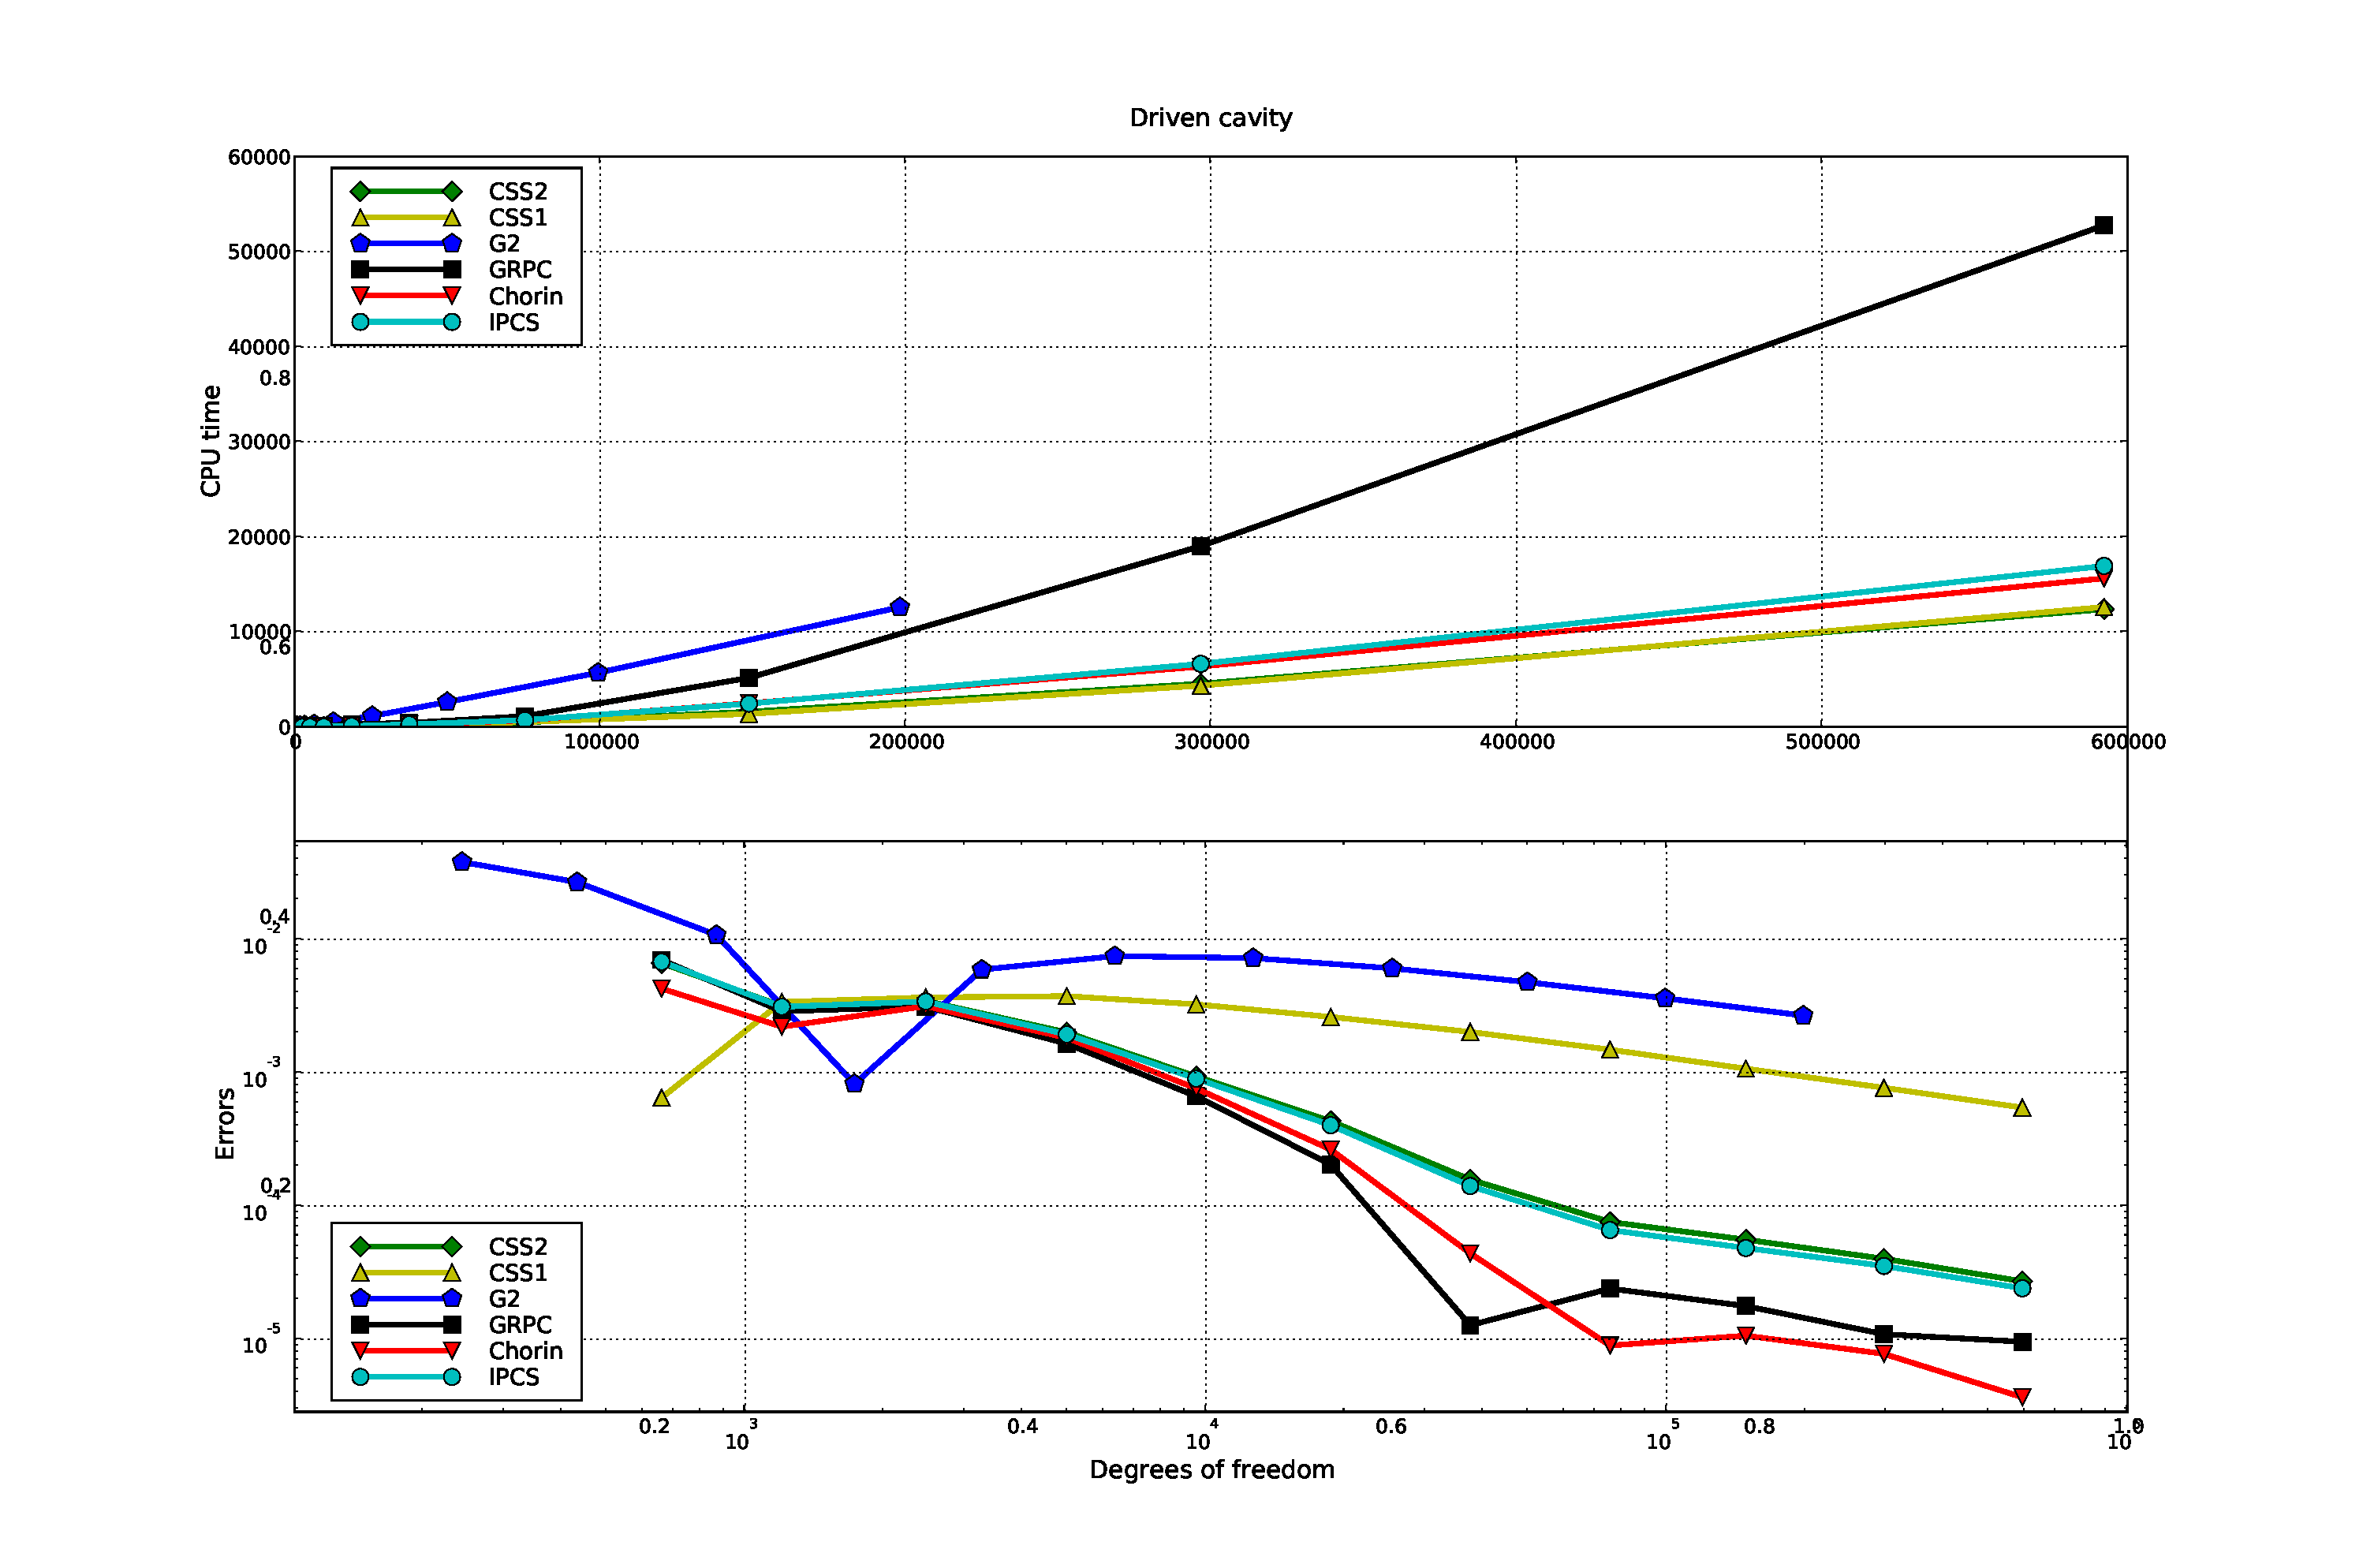
\includegraphics[width=20cm,height=11cm,keepaspectratio=false]{chapters/kvs-1/pdf/new_drivencavity_res.pdf}
  \caption{Results for the driven cavity test problem.}
  \label{fig:drivencavity_CPU_and_errors}
\end{figure*}

\subsection{Pressure-driven channel flow (2D)}

As a second test problem, we seek the solution of the Navier--Stokes
equations in a two-dimensional pressure-driven channel. The geometry
of the channel is the unit square $[0, 1]^2$ and the kinematic
viscosity is $\nu = 1/8$. No-slip boundary conditions are applied to
the velocity at the upper and lower walls and Neumann boundary
conditions are applied at the inlet and outlet. Dirichlet boundary
conditions are applied to the pressure at the inlet and outlet, with
$p = 1$ at the inlet and $p = 0$ at the outlet. The initial condition
is $u = (0, 0)$ for the velocity. As a functional of interest, we
consider the $x$-component of the velocity at $(x, y) = (1, 0.5)$ at
final time $T = 0.5$. By a Fourier series expansion, it is easy to
show that the exact value of the velocity at this point is given by
\begin{equation} \label{eq:exact_channel}
  u_x(1, 0.5, t) = 1 - \sum_{n=1,3,...}^\infty \frac{32}{\pi^3 n^3}
  e^{-\frac{\pi^2 n^2 t}{8}} (-1)^{(n-1)/2}.
\end{equation}
At final time $T=0.5$, this values is $u_x(1, 0.5, 0.5) \approx
0.44321183655681595$.

\paragraph{Results.}

Figure~\ref{fig:channel_results} shows the results for the
pressure-driven channel test problem. Again, the smallest error is
obtained with the GRPC solver, closely followed by the IPCS solver.
The W-shaped curve for the G2 solver is an effect of the $\mathcal{P}_1$--$\mathcal{P}_1$
discretization which results in a vertex located at $(x, y) = (1,
0.5)$ only for every other refinement level.

\begin{figure*}
  \vspace{0.2cm}
  \hspace{-2cm}
  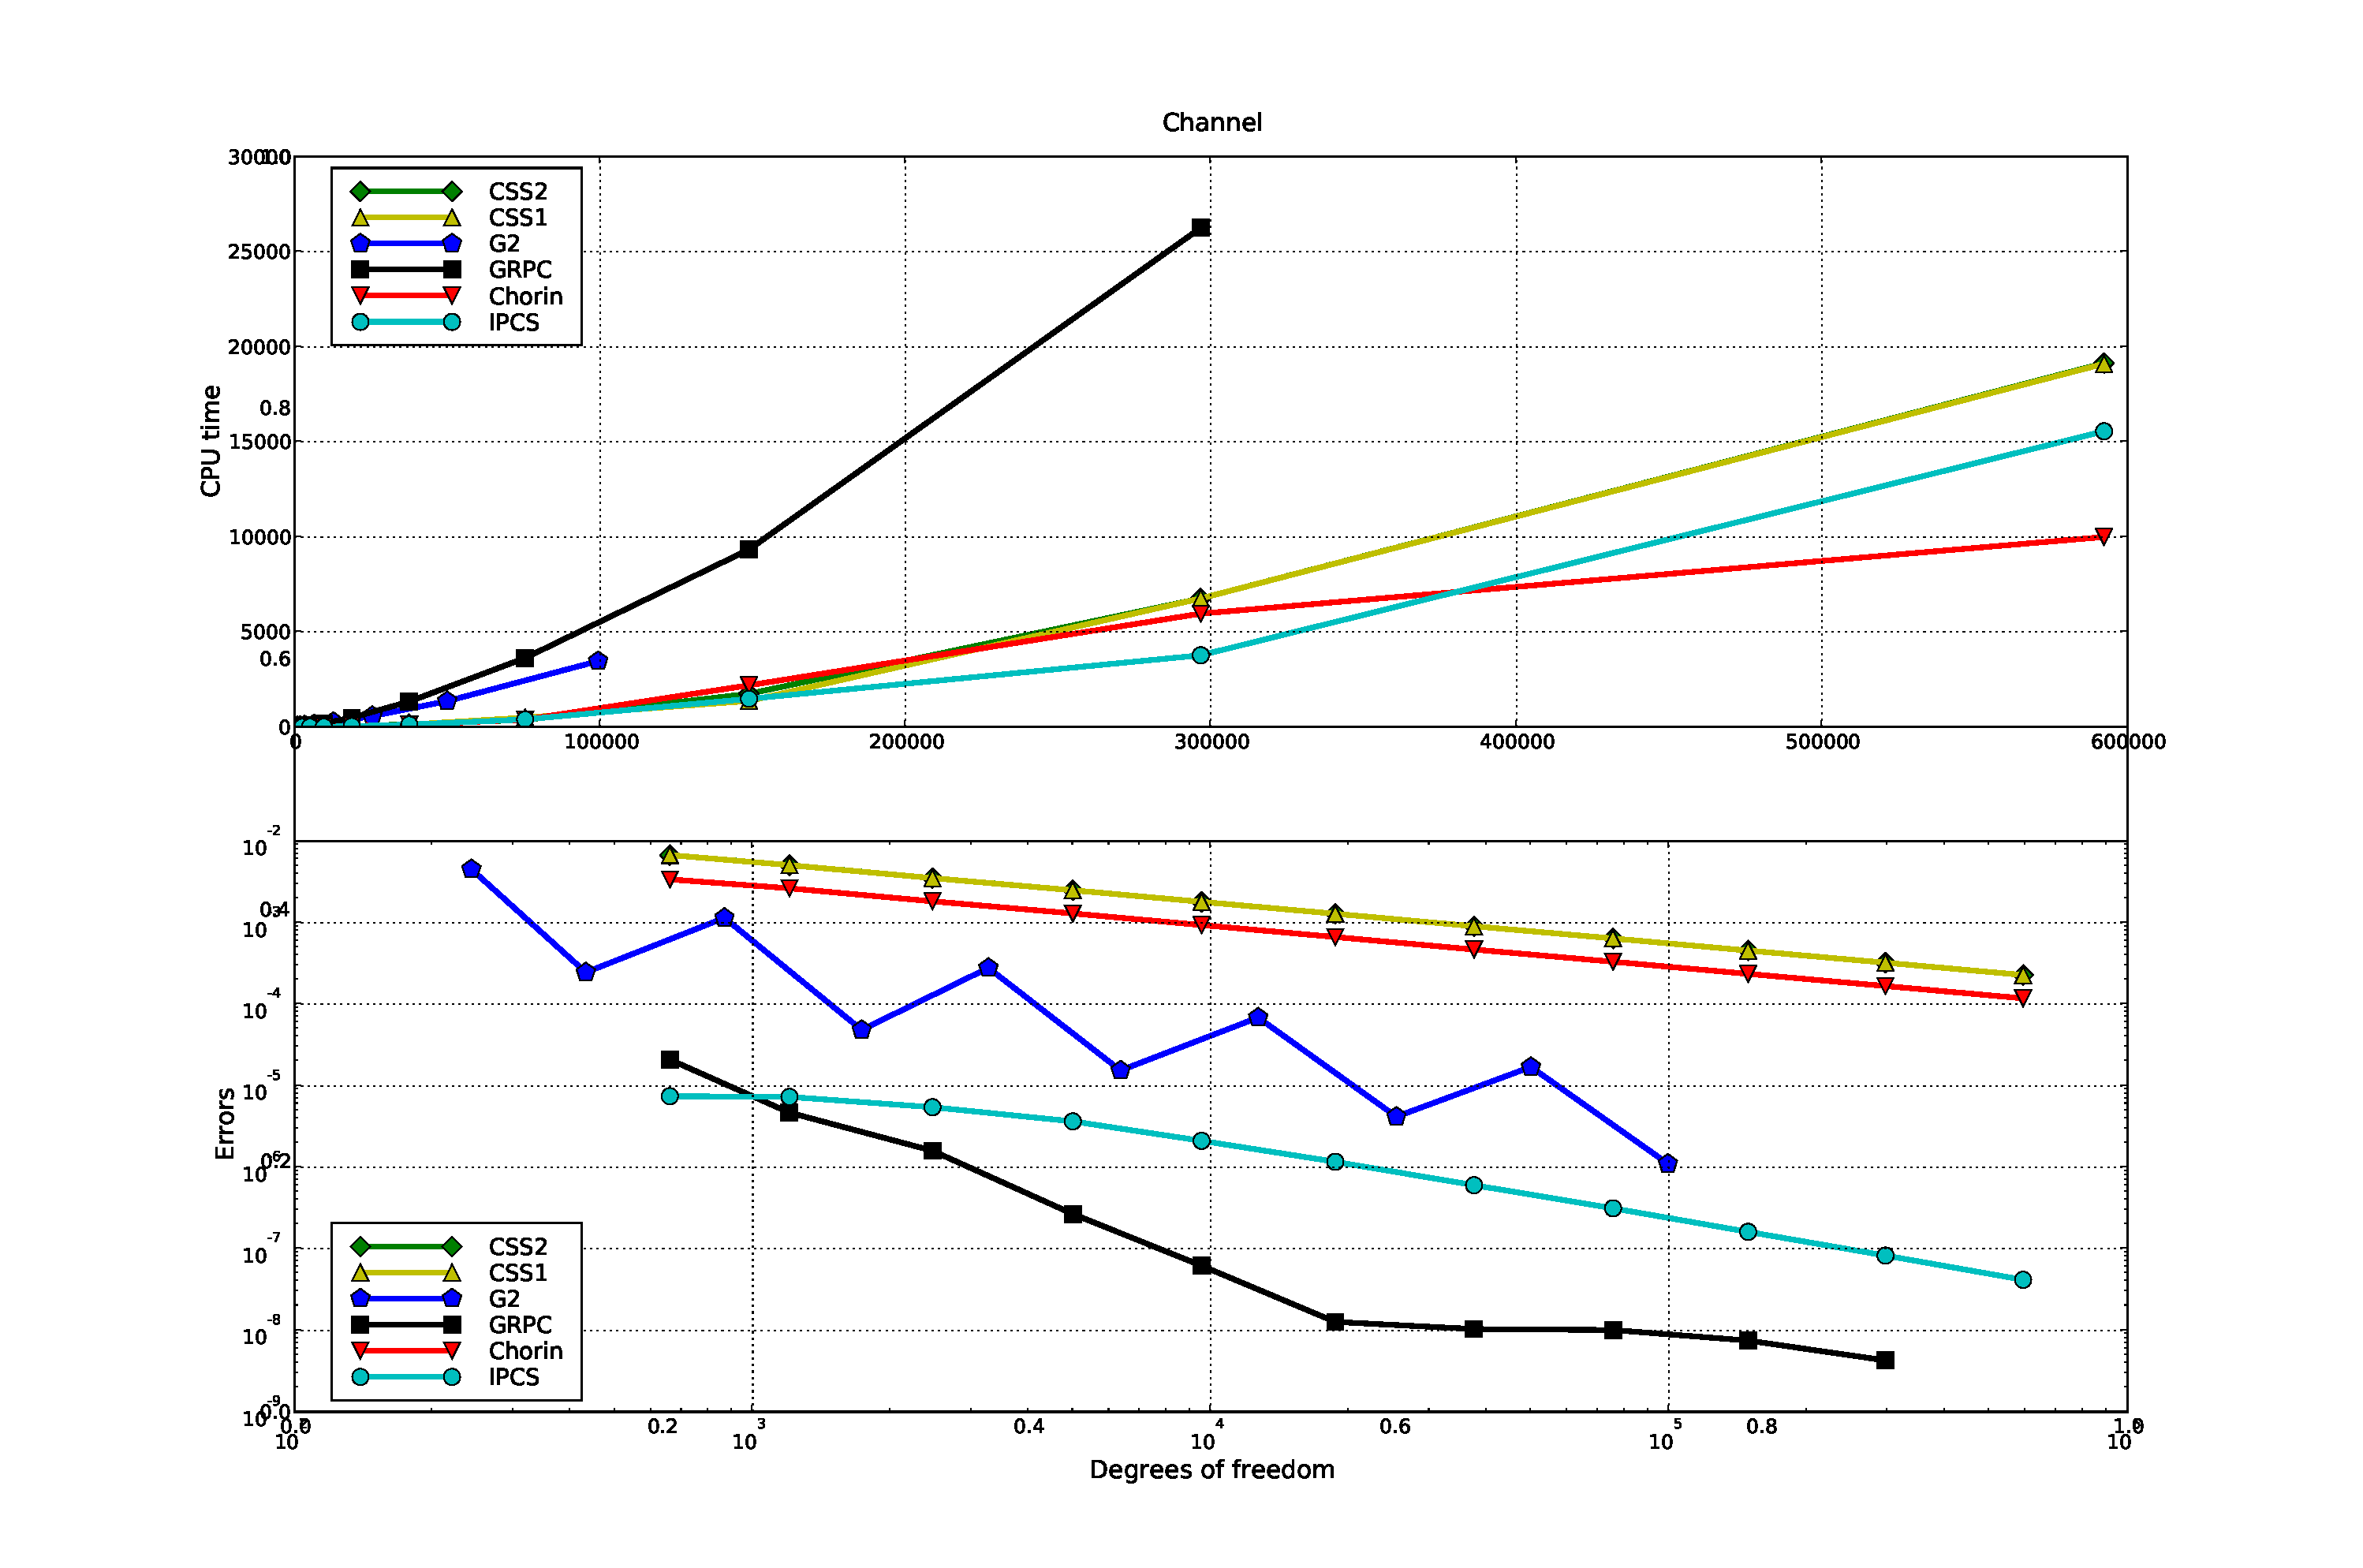
\includegraphics[width=20cm,height=11cm,keepaspectratio=false]{chapters/kvs-1/pdf/new_channel_res.pdf}
  \caption{Results for the pressure-driven channel test problem.}
  \label{fig:channel_results}
\end{figure*}

\subsection{Taylor--Green vortex (2D)}

As our next test problem, we consider the Taylor--Green vortex
described in \citet{CanutoHussainiQuarteroniEtAl2007}, which is a
periodic flow with exact solution given by
\begin{equation}\label{eq:periodic}
  \begin{split}
    u(x,y,t) = & (\cos (\pi x) \sin (\pi y)  e^{-2t\nu\pi^2}, \cos (\pi y)  \sin (\pi x)  e^{-2t\nu\pi^2}), \\
    p(x,y,t) = & -0.25(\cos(2\pi x ) + \cos(2\pi y ))  e^{-4t\nu\pi^2},
  \end{split}
\end{equation}
on the domain $[-1, 1]^{2}$. The kinematic viscosity is set to $\nu =
1/100$. Periodic boundary conditions are imposed in both the $x$ and
$y$ directions. The implementation of these boundary conditions in
DOLFIN is shown in Figure~\ref{fig:periodic_bcs}. The initial velocity
and pressure fields are shown in Figure~\ref{fig:periodic}. As a
functional of interest, we measure the kinetic energy $K = \frac{1}{2}
\|u\|^2_{L^2}$ at final time $T = 0.5$.

\begin{figure}
  %\codesize
  \begin{center}
    \begin{python}
class PeriodicBoundaryX(SubDomain):
    def inside(self, x, on_boundary):
        return x[0] < (-1.0 + DOLFIN_EPS) and \
               x[0] > (-1.0 - DOLFIN_EPS) and \
               on_boundary

    def map(self, x, y):
        y[0] = x[0] - 2.0
        y[1] = x[1]

class PeriodicBoundaryY(SubDomain):
    def inside(self, x, on_boundary):
        return x[1] < (-1.0 + DOLFIN_EPS) and \
               x[1] > (-1.0 - DOLFIN_EPS) and \
               on_boundary

    def map(self, x, y):
        y[0] = x[0]
        y[1] = x[1] - 2.0
    \end{python}
    \caption{Implementation of periodic boundary conditions for the
      Taylor--Green vortex test problem.}
    \label{fig:periodic_bcs}
  \end{center}
\end{figure}

\paragraph{Results.}

Figure~\ref{fig:periodic_res} shows the results for the Taylor--Green
test problem. The smallest error is obtained with the IPCS solver. For
this test problem, the G2 solver is overly dissipative and produces an
error which is six orders of magnitude larger than that of the IPCS
solver.

\begin{figure}
  \begin{center}
    \fbox{
      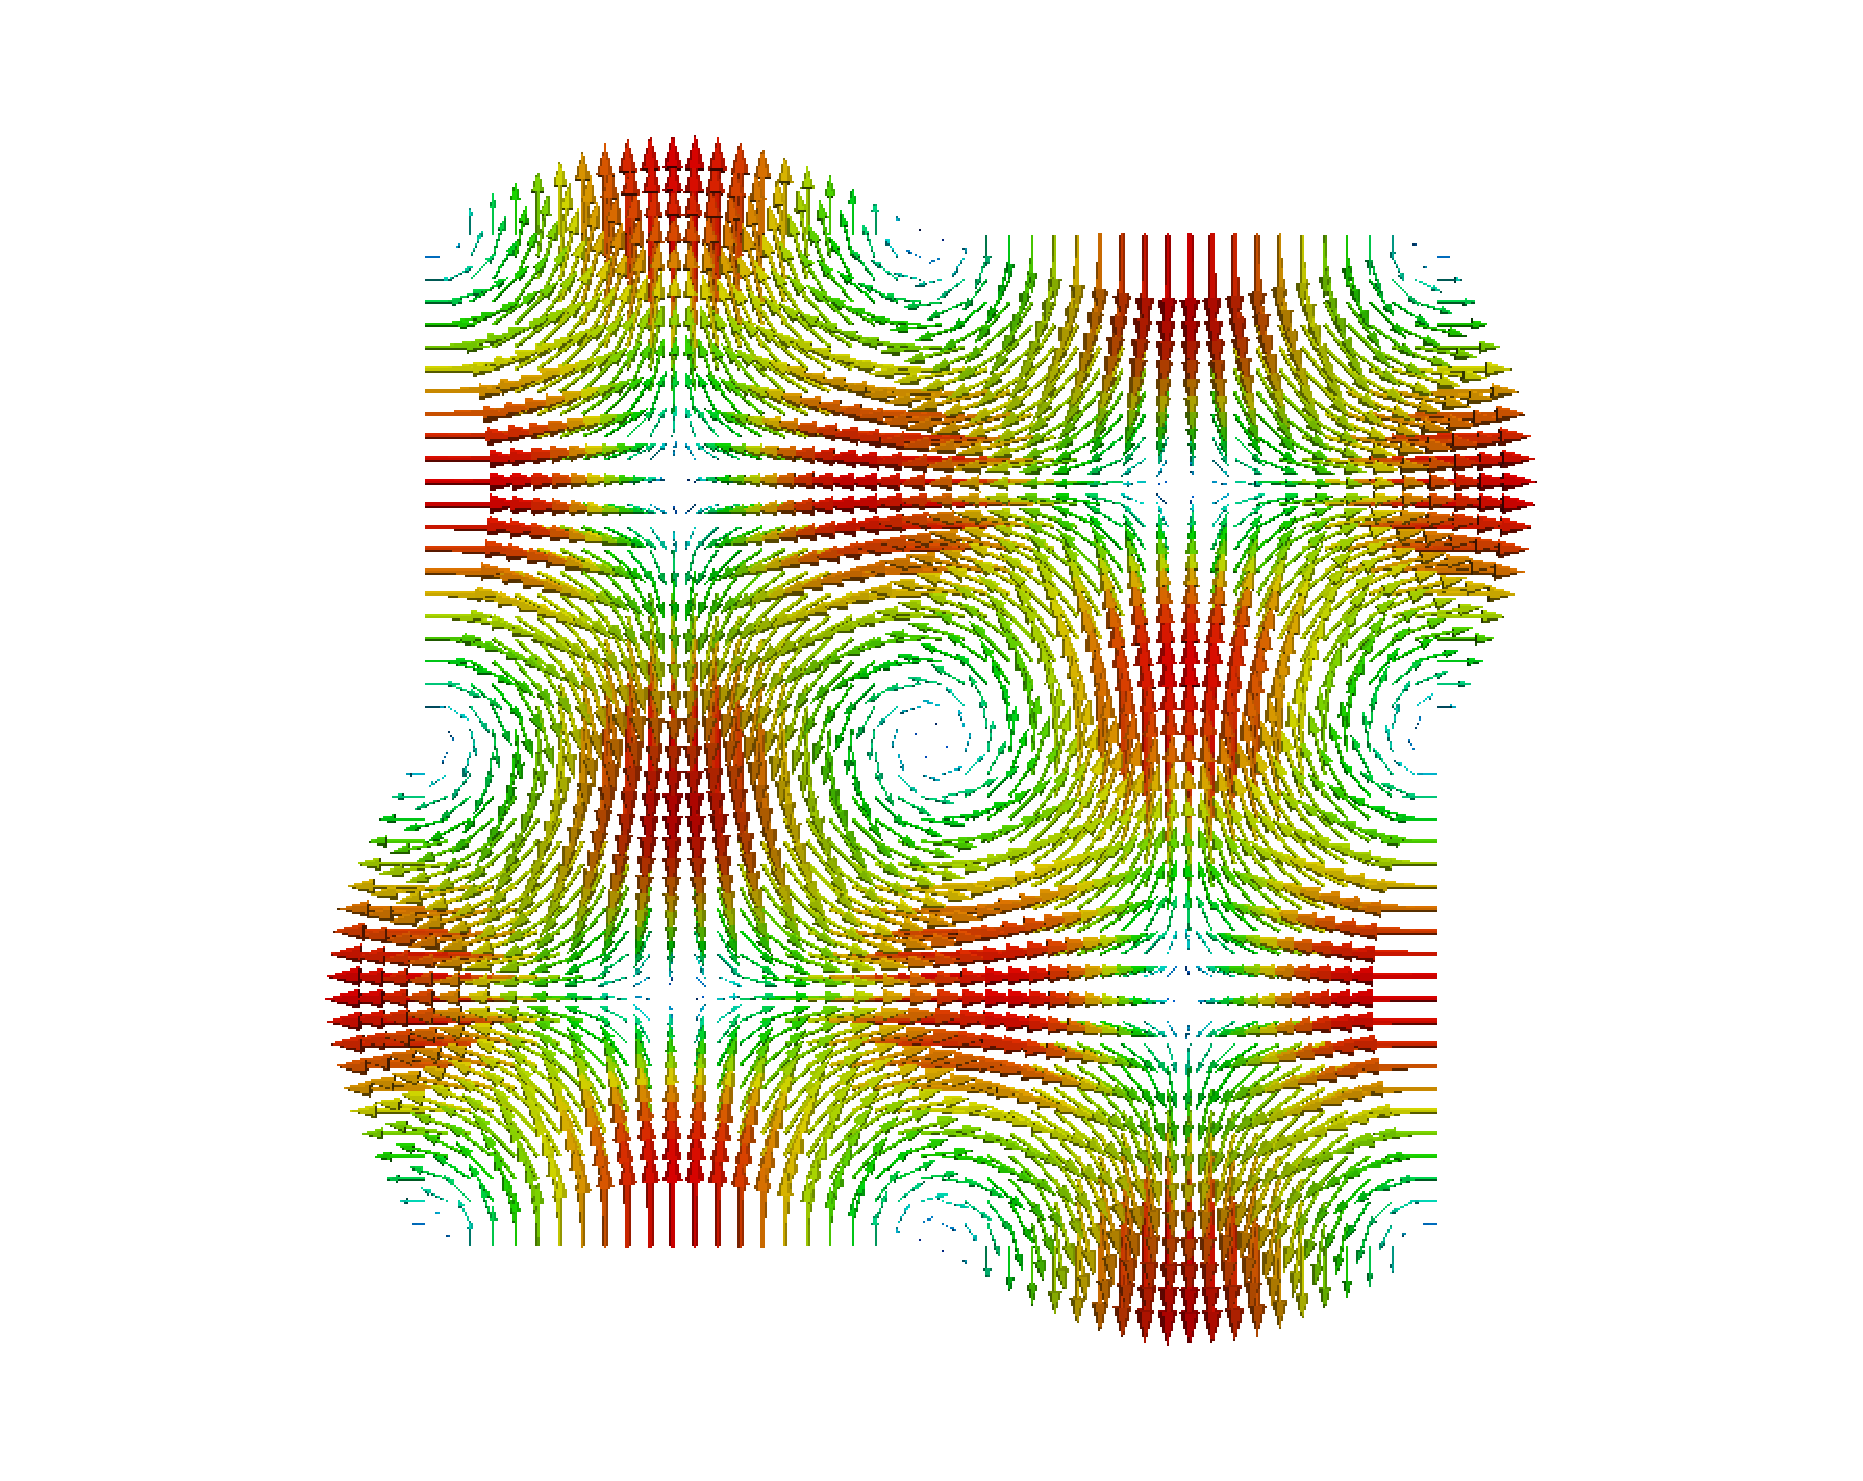
\includegraphics[width=5cm]{chapters/kvs-1/pdf/periodic_v.pdf}
      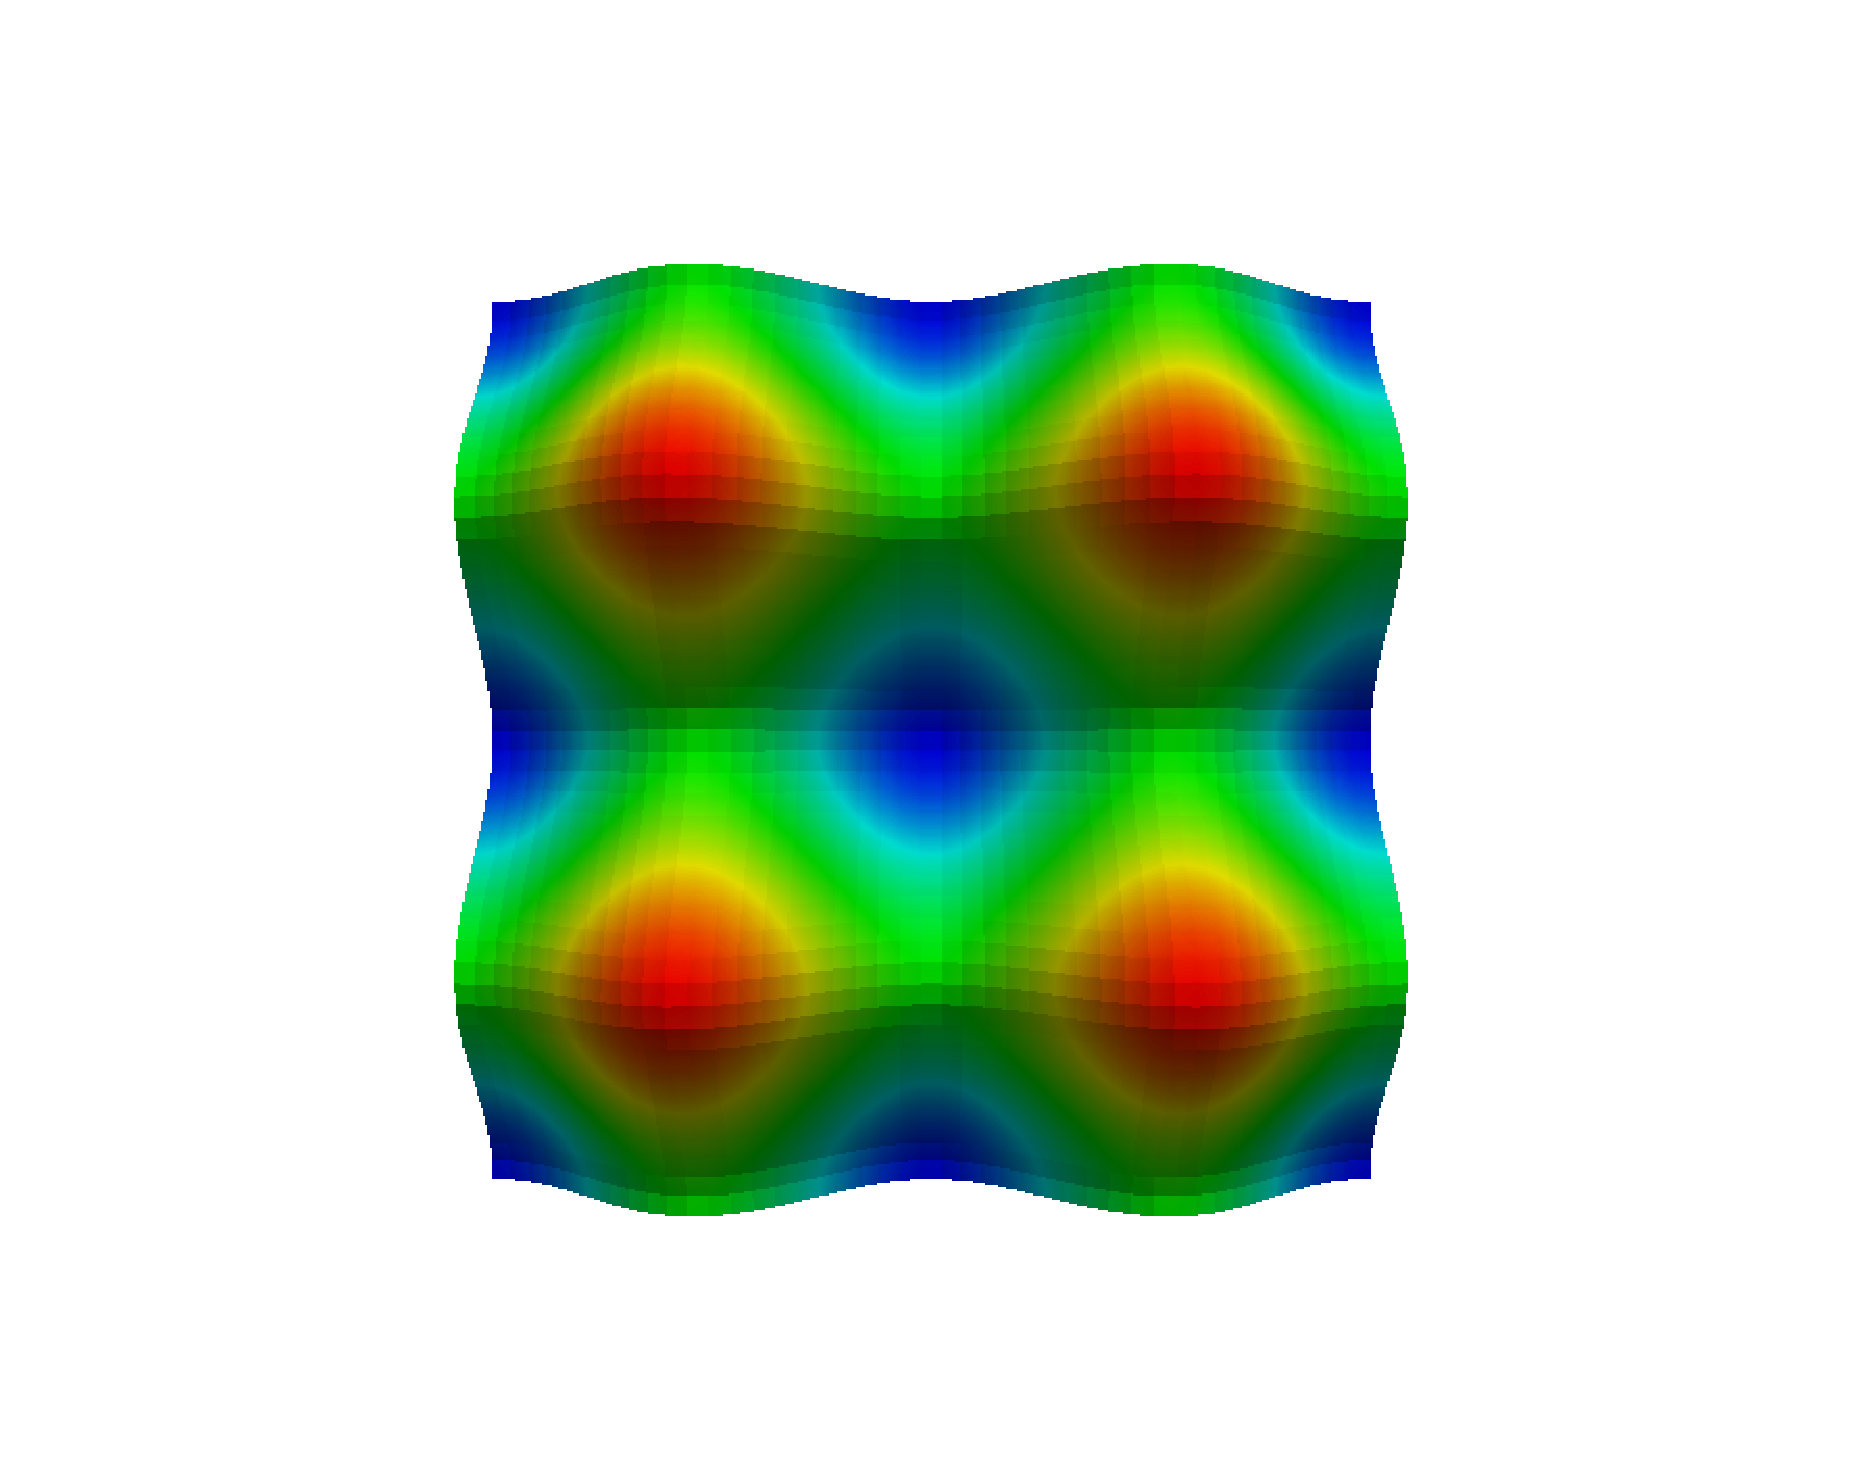
\includegraphics[width=5cm]{chapters/kvs-1/pdf/periodic_p.pdf}
    }
    \caption{An illustration of the initial conditions for the Taylor--Green vortex test
      problem. On the left is the velocity field with vectors and on
      the right is the corresponding pressure field.}
    \label{fig:periodic}
  \end{center}
\end{figure}

\begin{figure*}
  \hspace{-2cm}
  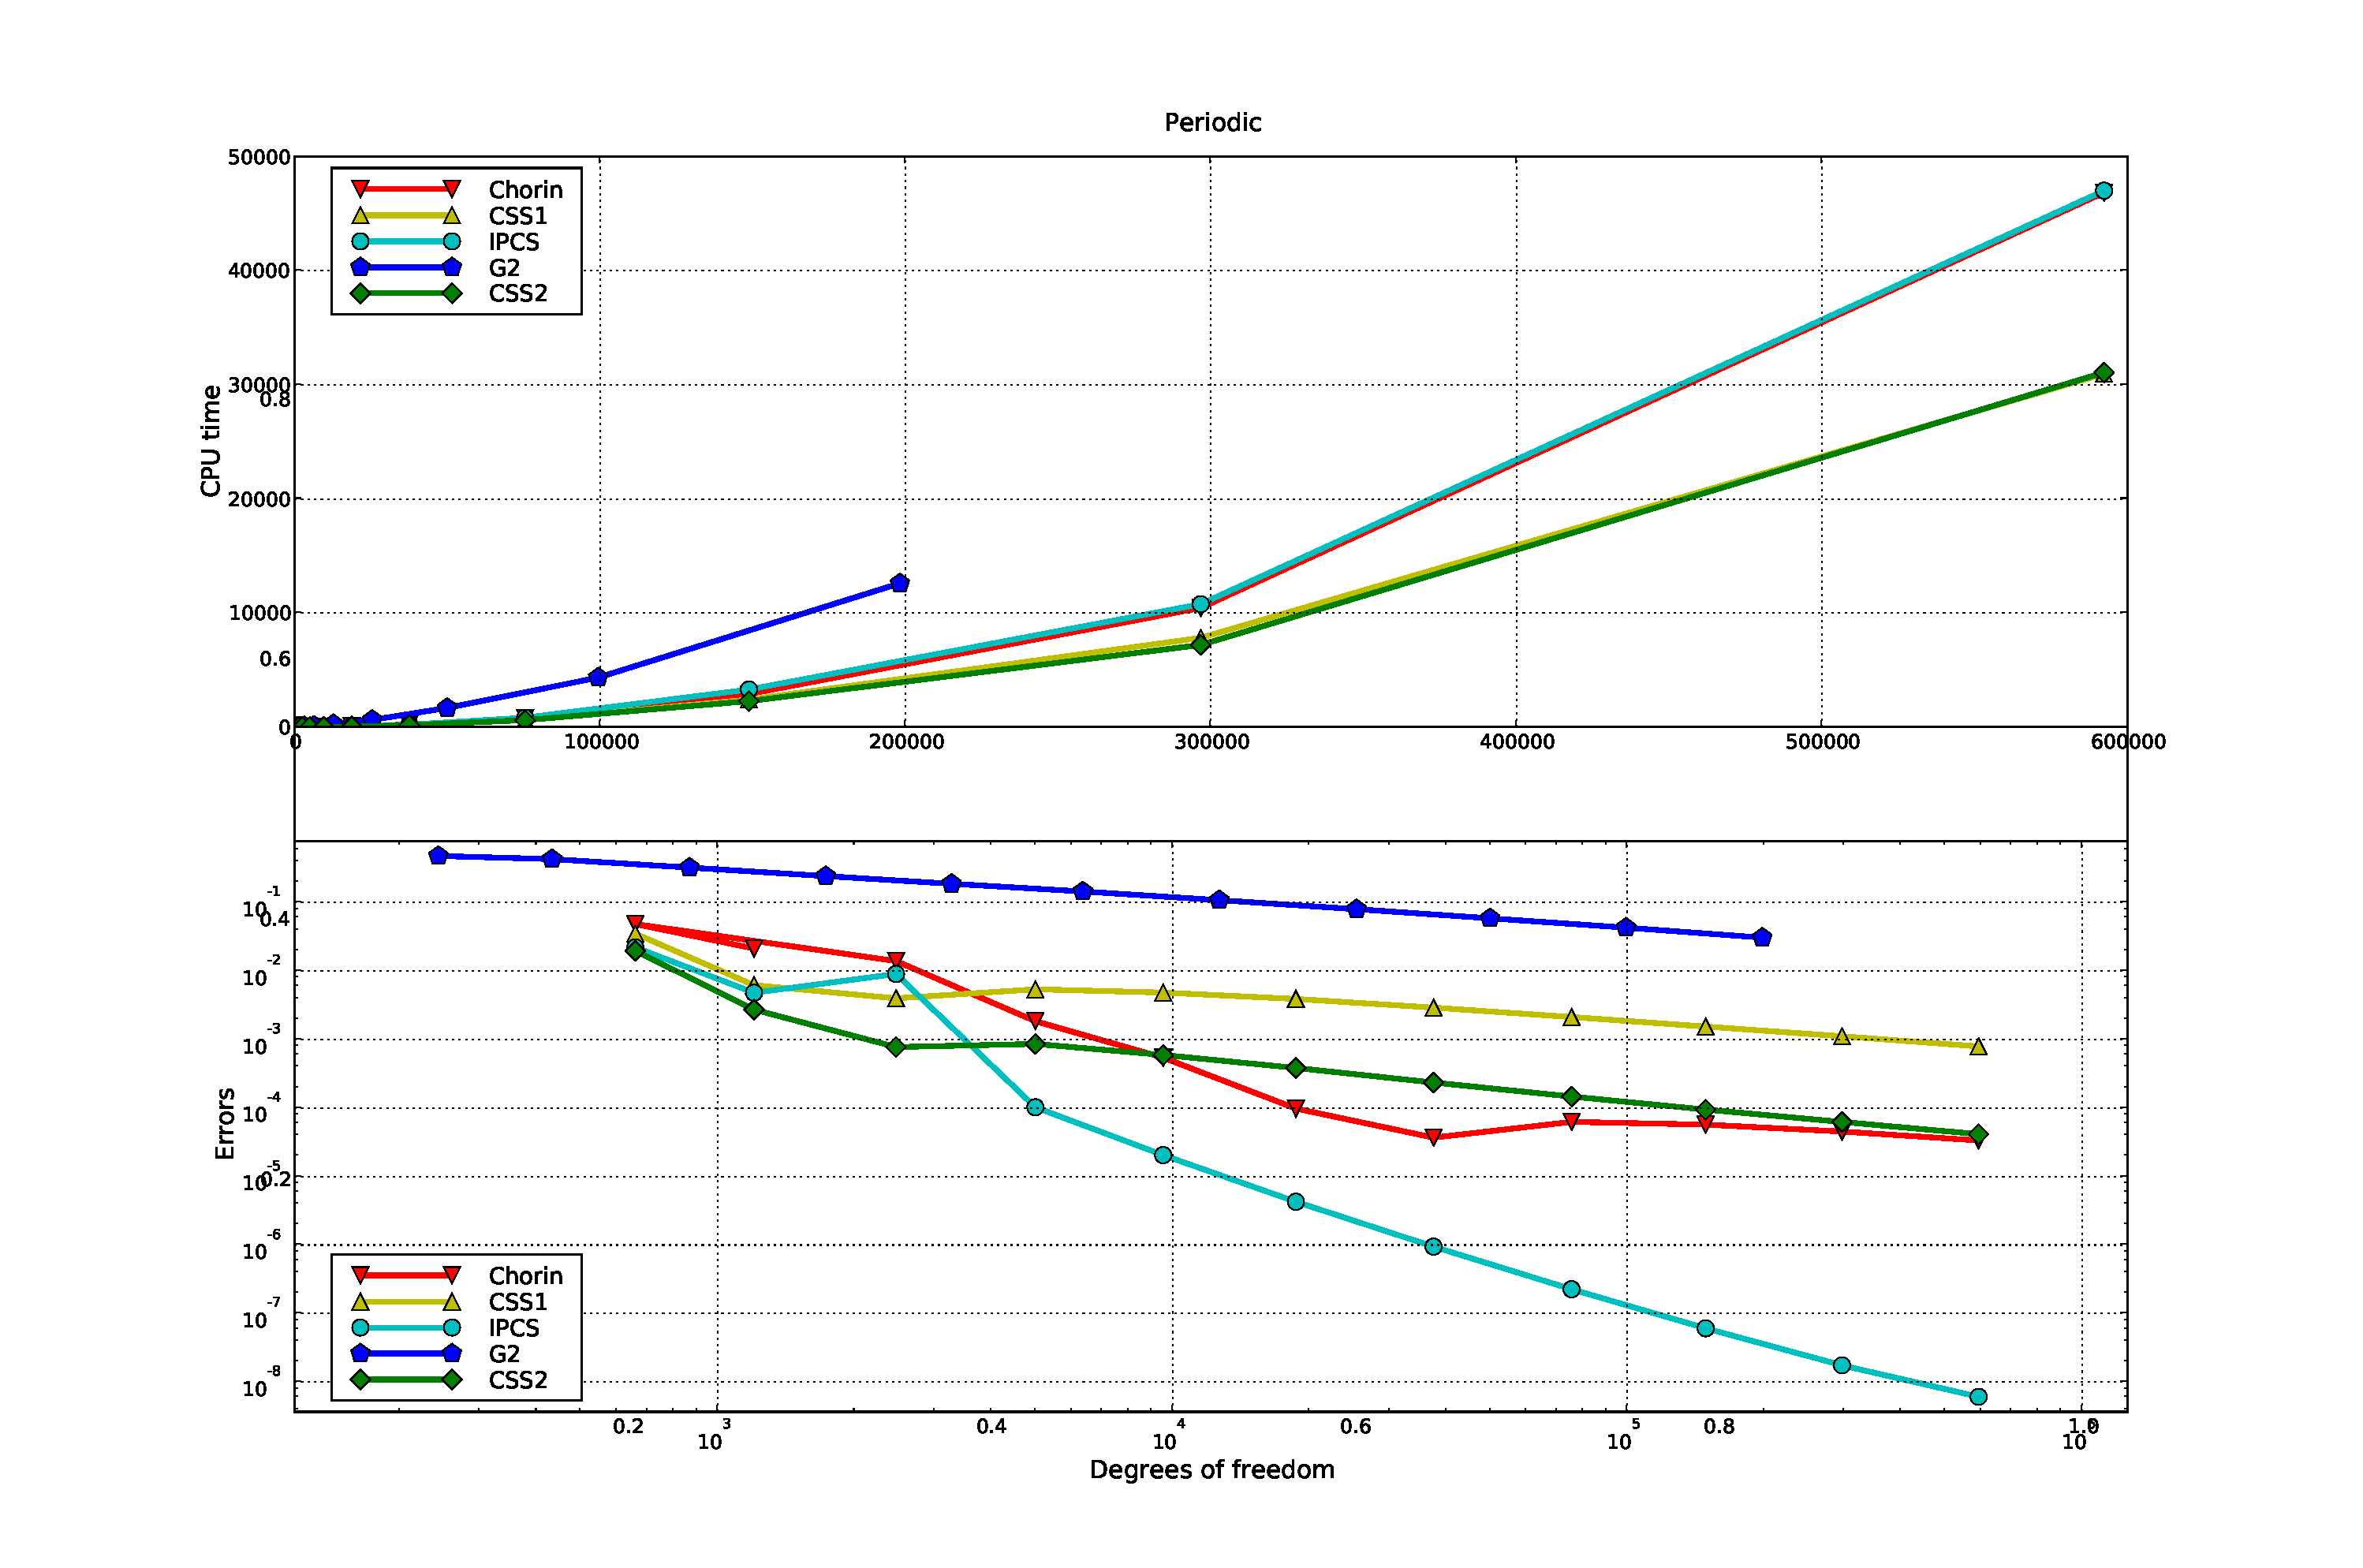
\includegraphics[width=20cm,height=11cm,keepaspectratio=false]{chapters/kvs-1/pdf/new_periodic_res.pdf}
  \caption{Results for the Taylor--Green vortex test problem.}
  \label{fig:periodic_res}
\end{figure*}

\subsection{Flow past a cylinder (2D)}

We next consider a test problem from \citet{Turek1996}, which is a
two-dimensional cylinder submerged into a fluid and surrounded by
solid walls as illustrated in
Figure~\ref{fig:cylinder_illustration}. The cylinder is slightly
displaced from the center of the channel and the resulting flow is a
vortex street forming behind the cylinder. No-slip boundary conditions
are applied to the cylinder as well as the upper and lower walls of
the channel. A zero Dirichlet boundary condition is imposed on the
pressure at the outlet. The inflow velocity is a time-varying
parabolic profile given by
\begin{equation} \label{eq:cyl_inflow}
  u(0, y, t) = (4 U_m y (H - y) \sin(\pi t/8)/H^{4}, 0), \quad t \leqslant 8,
\end{equation}
where $U_m = 1.5$ and $H = 0.41$. The kinematic viscosity is $\nu =
1/1000$. As a functional of interest, we consider the pressure
difference between the front and back of the cylinder at final time $T
= 8$, that is,
\begin{equation}\label{eq:dp}
  \Delta p = p(0.45, 0.2, 8) - p(0.55, 0.2, 8).
\end{equation}
A reference value $-0.11144$ for this functional was obtained using
the IPCS solver on a mesh that was approximately of twice the size (in
terms of the number of cells) as the finest mesh used in the test,
with a time step of approximately half the size of the finest used
time step.

\begin{figure*}
  \center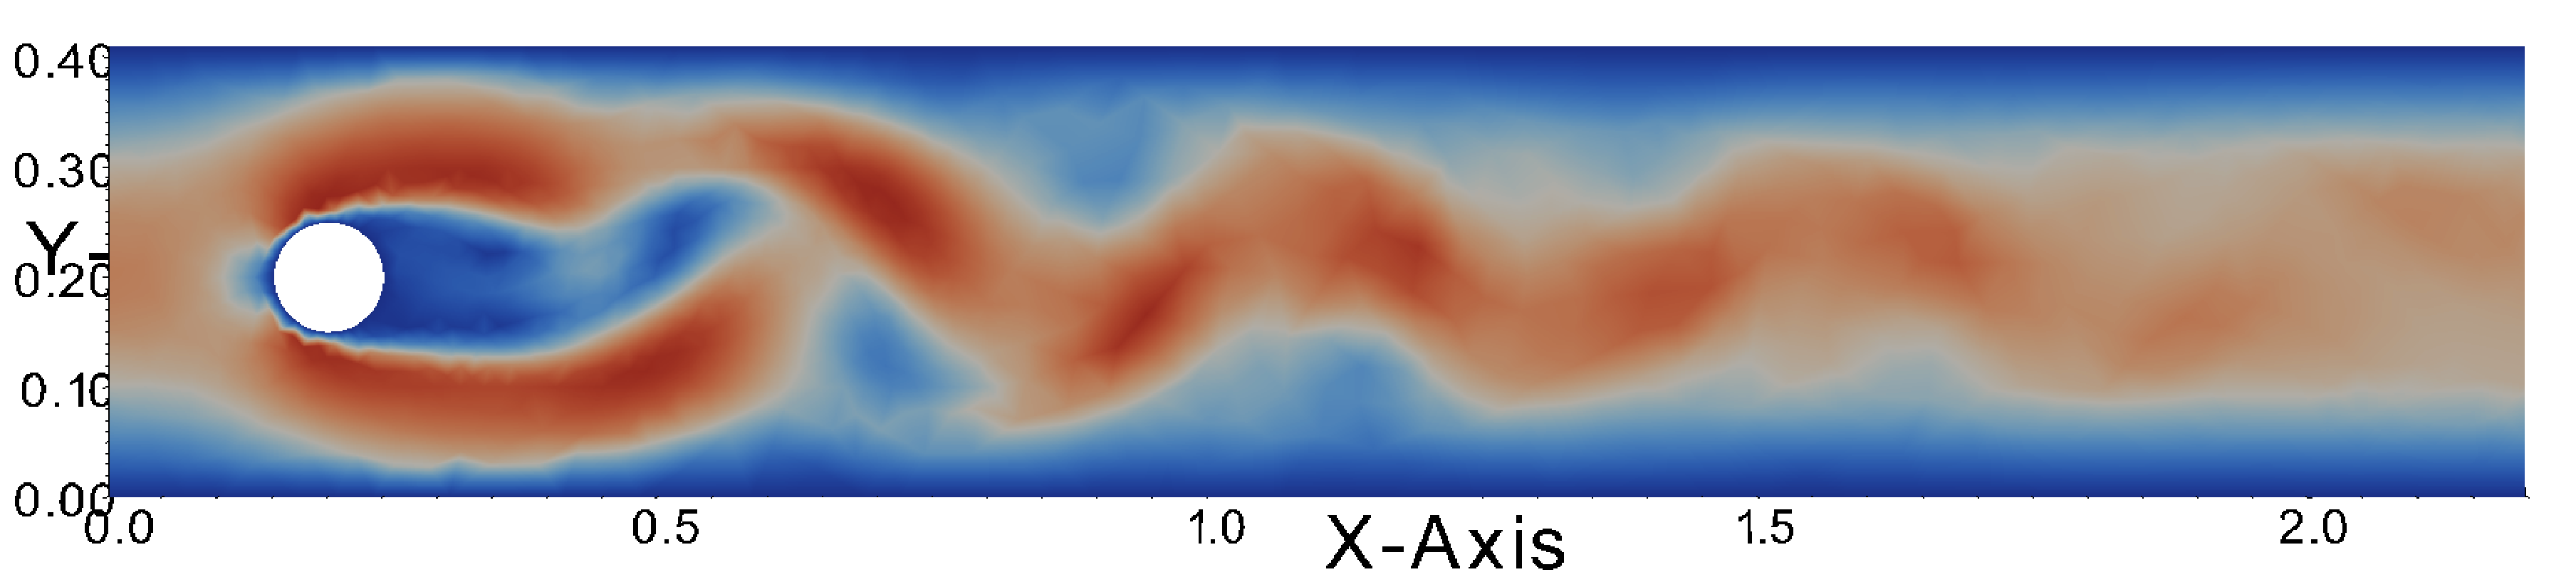
\includegraphics[width=\fullfig]{chapters/kvs-1/pdf/cylinderandgeoattime5nr2.pdf}
  \caption{Illustration of the velocity field for the cylinder test problem at $t = 5$.}
  \label{fig:cylinder_illustration}
\end{figure*}

\vspace{1cm}


\paragraph{Results.}

Figure~\ref{fig:cylinder_res} shows the results for the cylinder test
problem. The smallest error is obtained with the GRPC solver closely
followed by $\mathrm{CSS}_2$ and IPCS. It is interesting to note that
for this test problem, the $\mathrm{CSS}_2$ solver is also the
fastest.

\begin{figure*}
  \hspace{-2cm}
  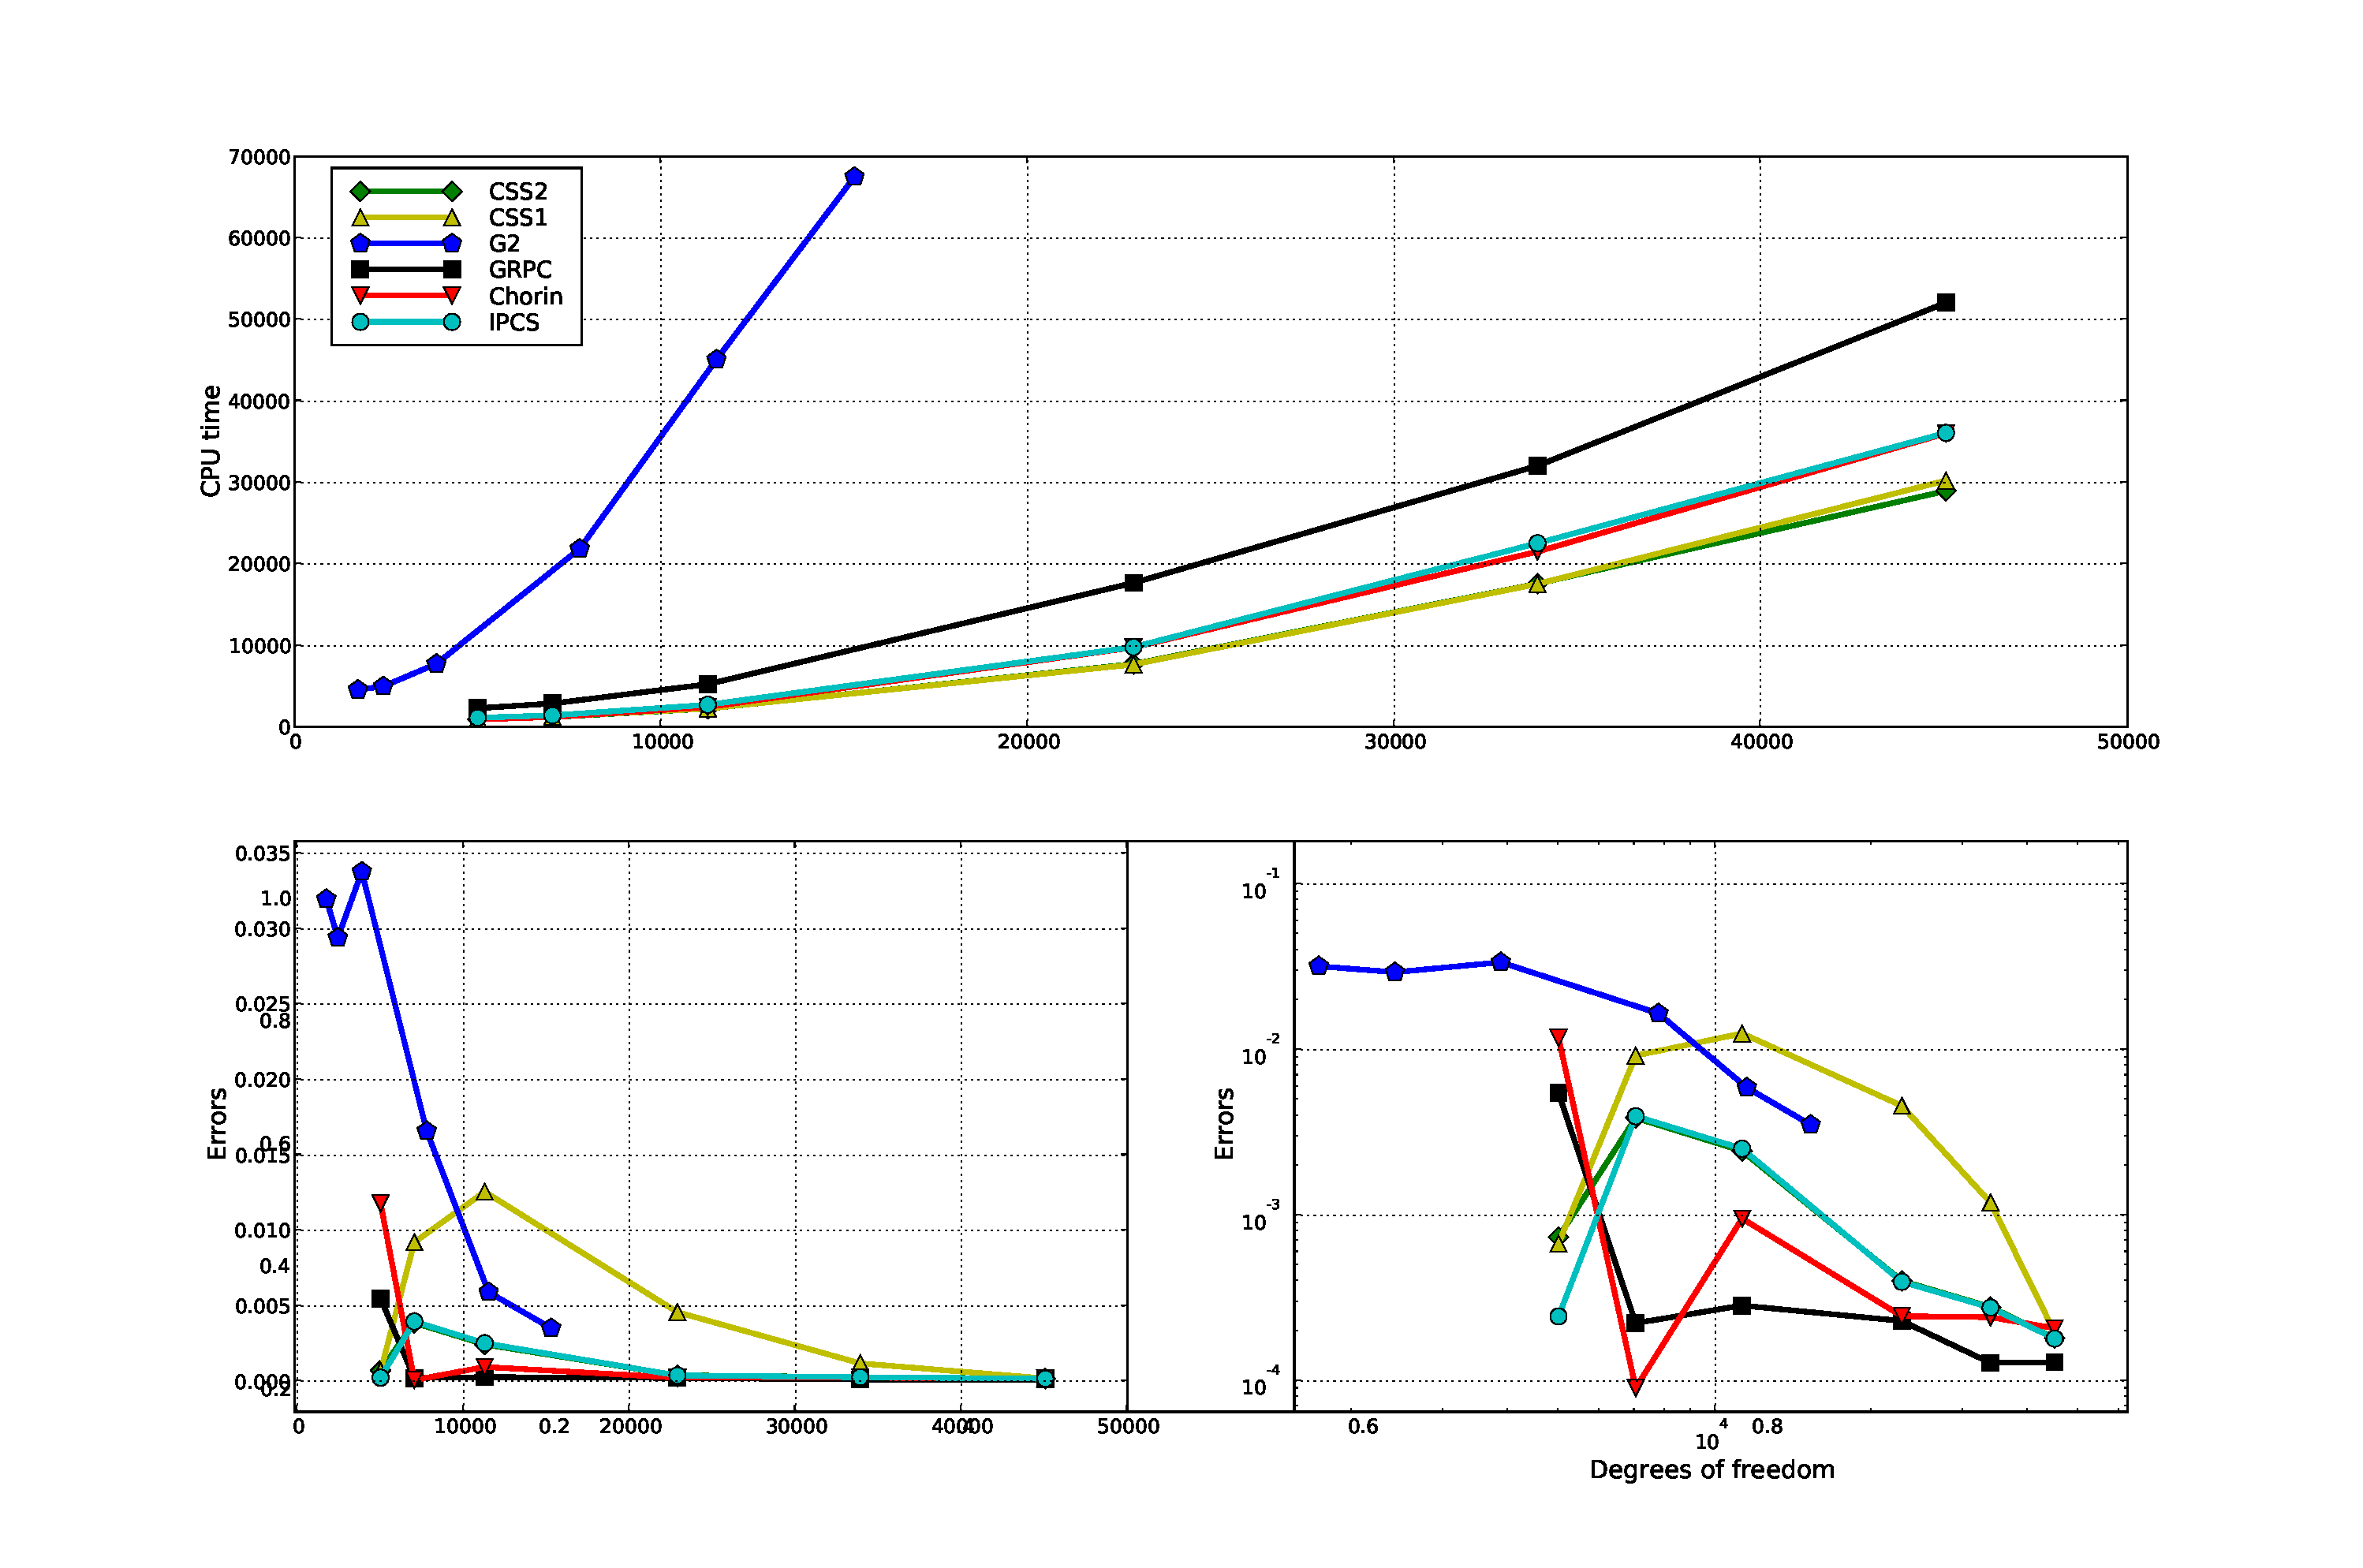
\includegraphics[width=20cm,height=11cm,keepaspectratio=false]{chapters/kvs-1/pdf/new_cylinder_res.pdf}
  \caption{Results for the cylinder test problem.}
  \label{fig:cylinder_res}
\end{figure*}

\subsection{Beltrami flow (3D)}

We next consider a problem described in \citet{EthierSteinmann1994}
where an exact fully three-dimensional solution of the Navier--Stokes
equations is derived. The flow is a so-called Beltrami flow, which has
the property that the velocity and vorticity vectors are aligned. The
domain is a cube with dimensions $[-1, 1]^3$. The exact velocity is
given by
\begin{equation}
  \begin{split}
    u(x,y,z,t) =& -a [ e^{a x} \sin(a y + d z)  + e^{az} \cos(a x + d y) ] e^{-d^{2}t}, \\
    v(x,y,z,t) =& -a [ e^{a y} \sin(a z + d x)  + e^{ax} \cos(a y + d z) ] e^{-d^{2}t}, \\
    w(x,y,z,t) =& -a [ e^{a z} \sin(a x + d y)  + e^{ay} \cos(a z + d x) ] e^{-d^{2}t},
  \end{split}
\end{equation}
and the exact pressure is given by
\begin{multline}
    p(x,y,z,t) = - a^2 e^{-2d^{2}t}
    \left(e^{2ax} + e^{2ay} + e^{2az}\right)
    \left(
    \sin(a x + d y) \cos(a z + d x) e^{a(y+z)} \right.
    \\
    \left. + \sin(a y + d z) \cos(a x + d y) e^{a(x+z)} +
    \sin(a z + d x) \cos(a y + d z) e^{a(x+y)}
    \right).
\end{multline}
The solution is visualized in Figure~\ref{fig:beltrami}. The constants
$a$ and $d$ may be chosen arbitrarily, and have been set to $a=\pi/4$
and $d=\pi/2$ as in \citet{EthierSteinmann1994}. The kinematic
viscosity is $\nu = 1$. To measure the error, we compute the $L^2$
norm of the error in the velocity field at final time $T = 0.5$
divided by the $L^2$ norm of the exact solution as
in \citet{EthierSteinmann1994}.

\begin{figure}
  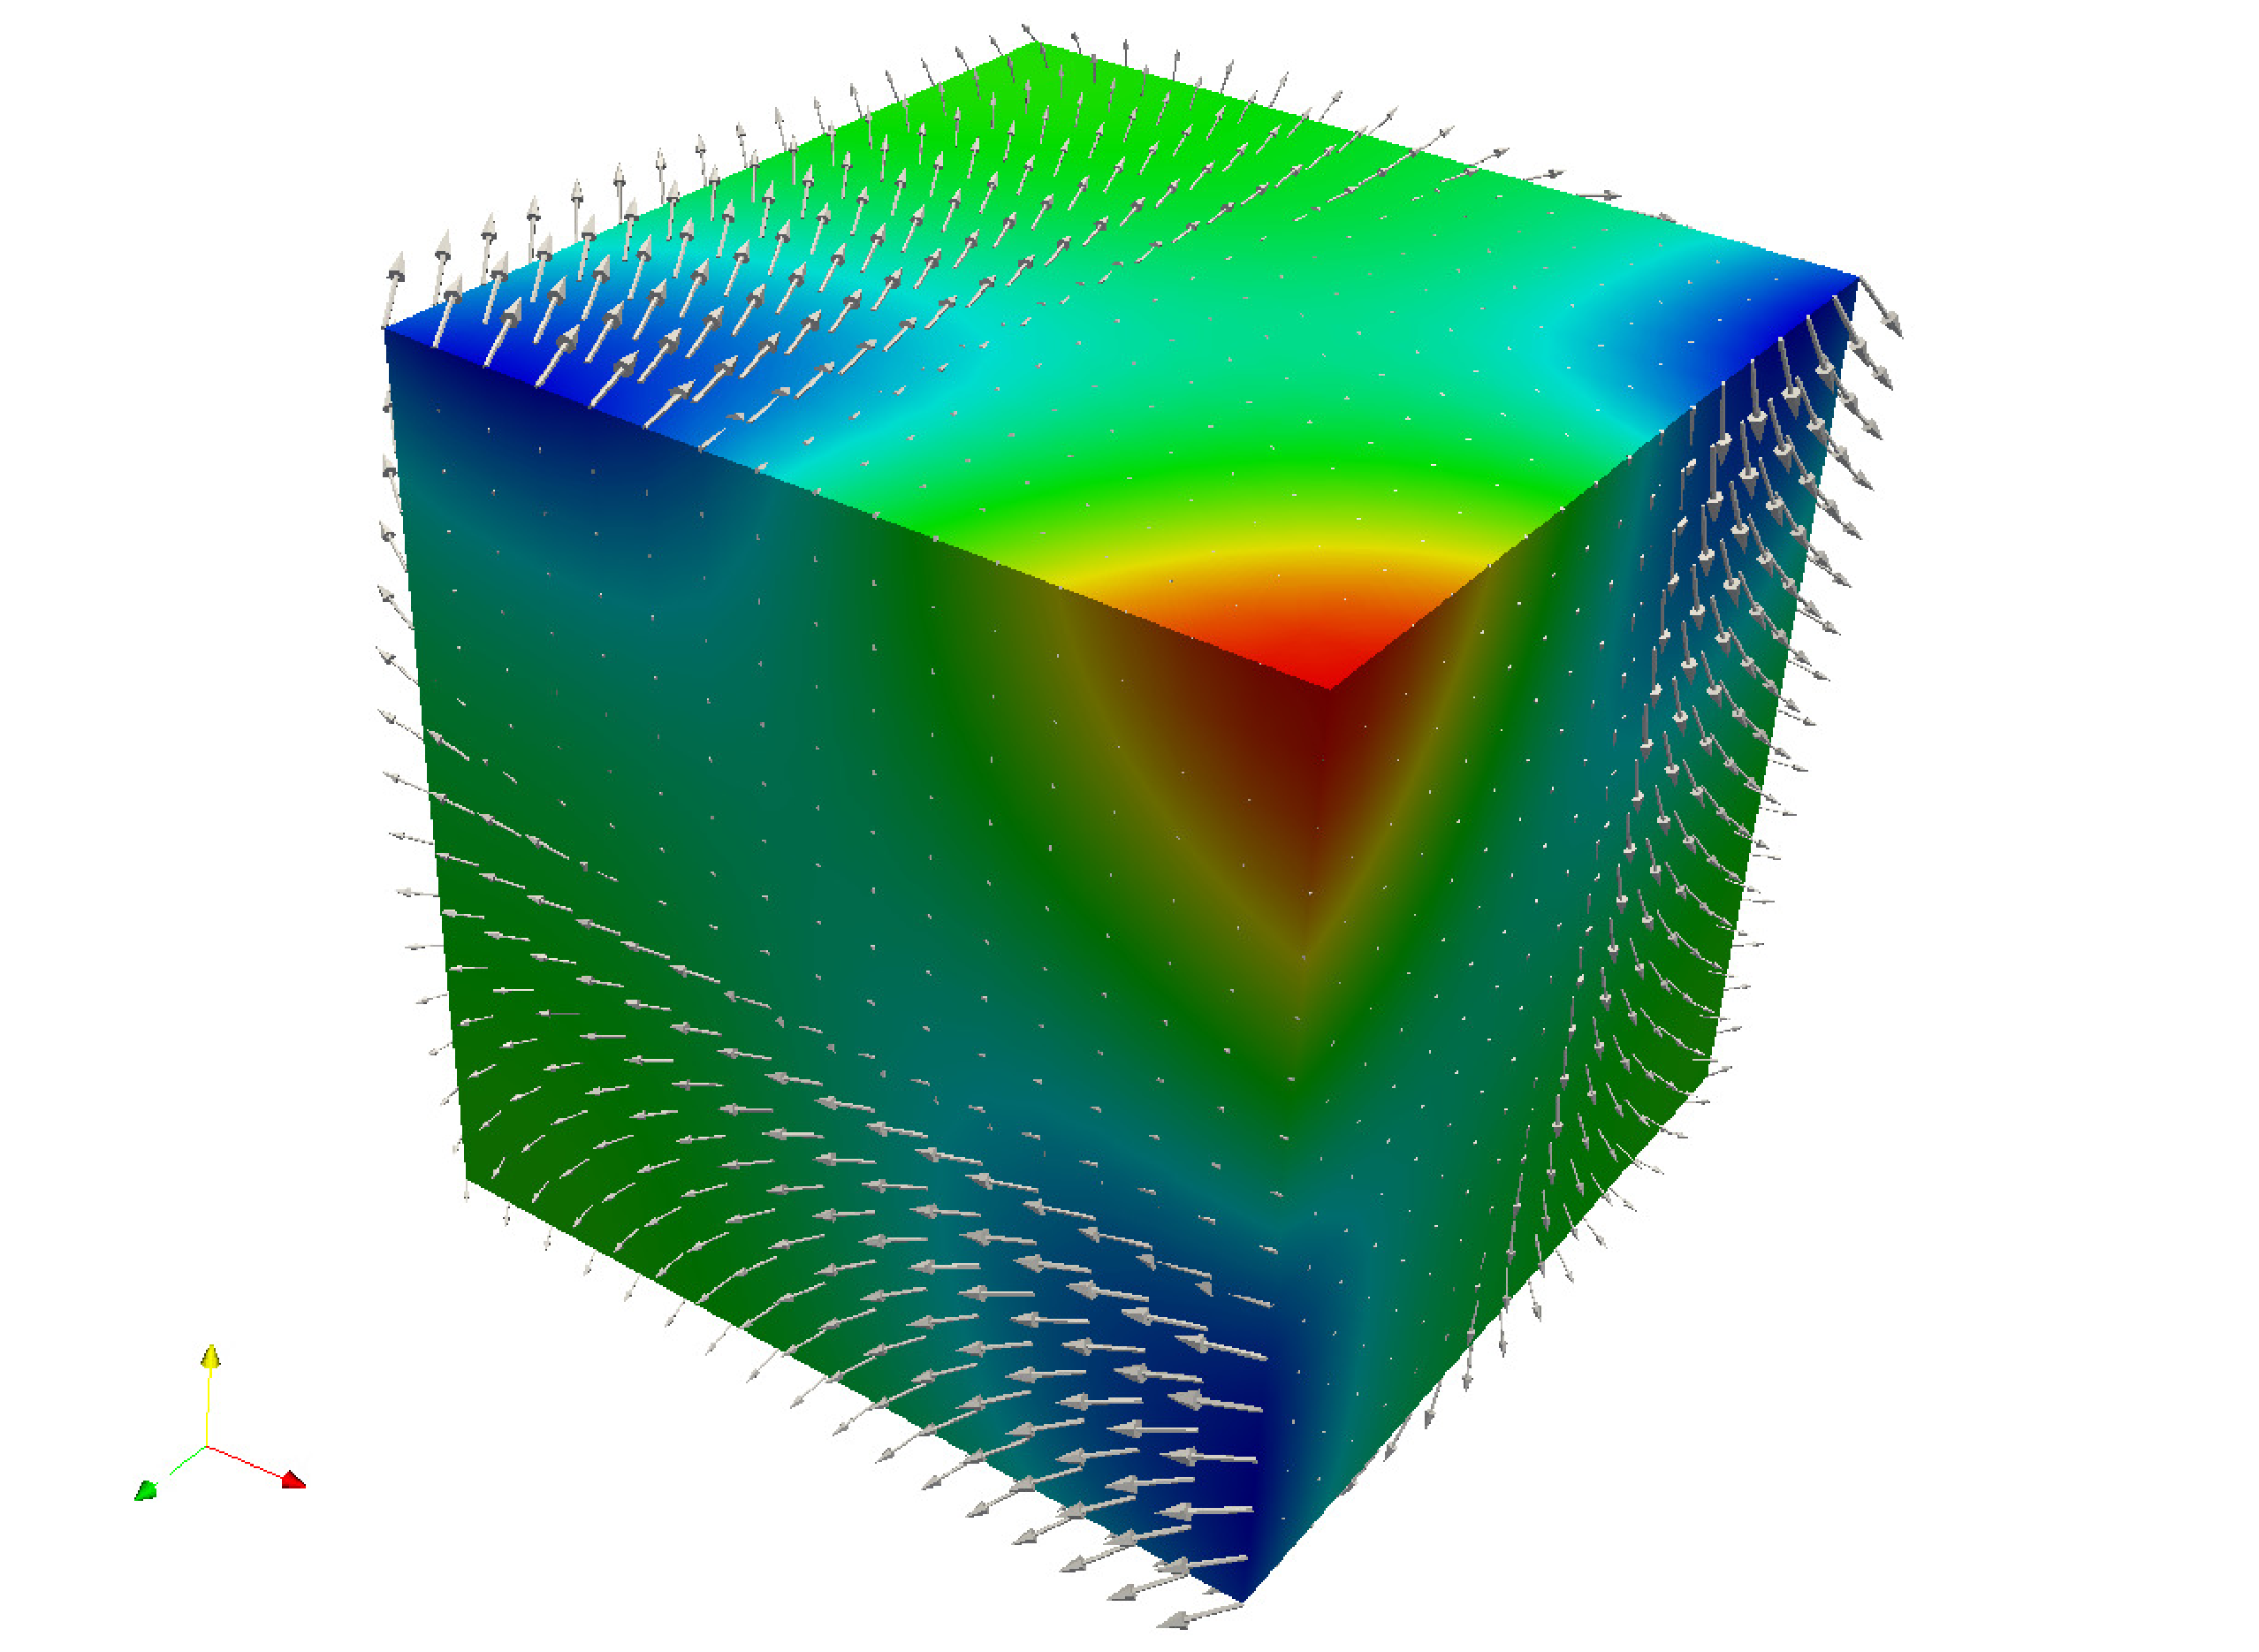
\includegraphics[width=\largefig]{chapters/kvs-1/pdf/new_beltrami_illustration.pdf}
  \caption{Solution of the Beltrami flow test problem.}
  \label{fig:beltrami}
\end{figure}

\paragraph{Results.}

Figure~\ref{fig:beltrami_res} shows the results for the Beltrami test
problem. The smallest errors are obtained with the GRPC solver, while
the largest errors are obtained with the $\mathrm{CSS}_1$ solver.

\begin{figure*}
  \hspace{-2cm}
  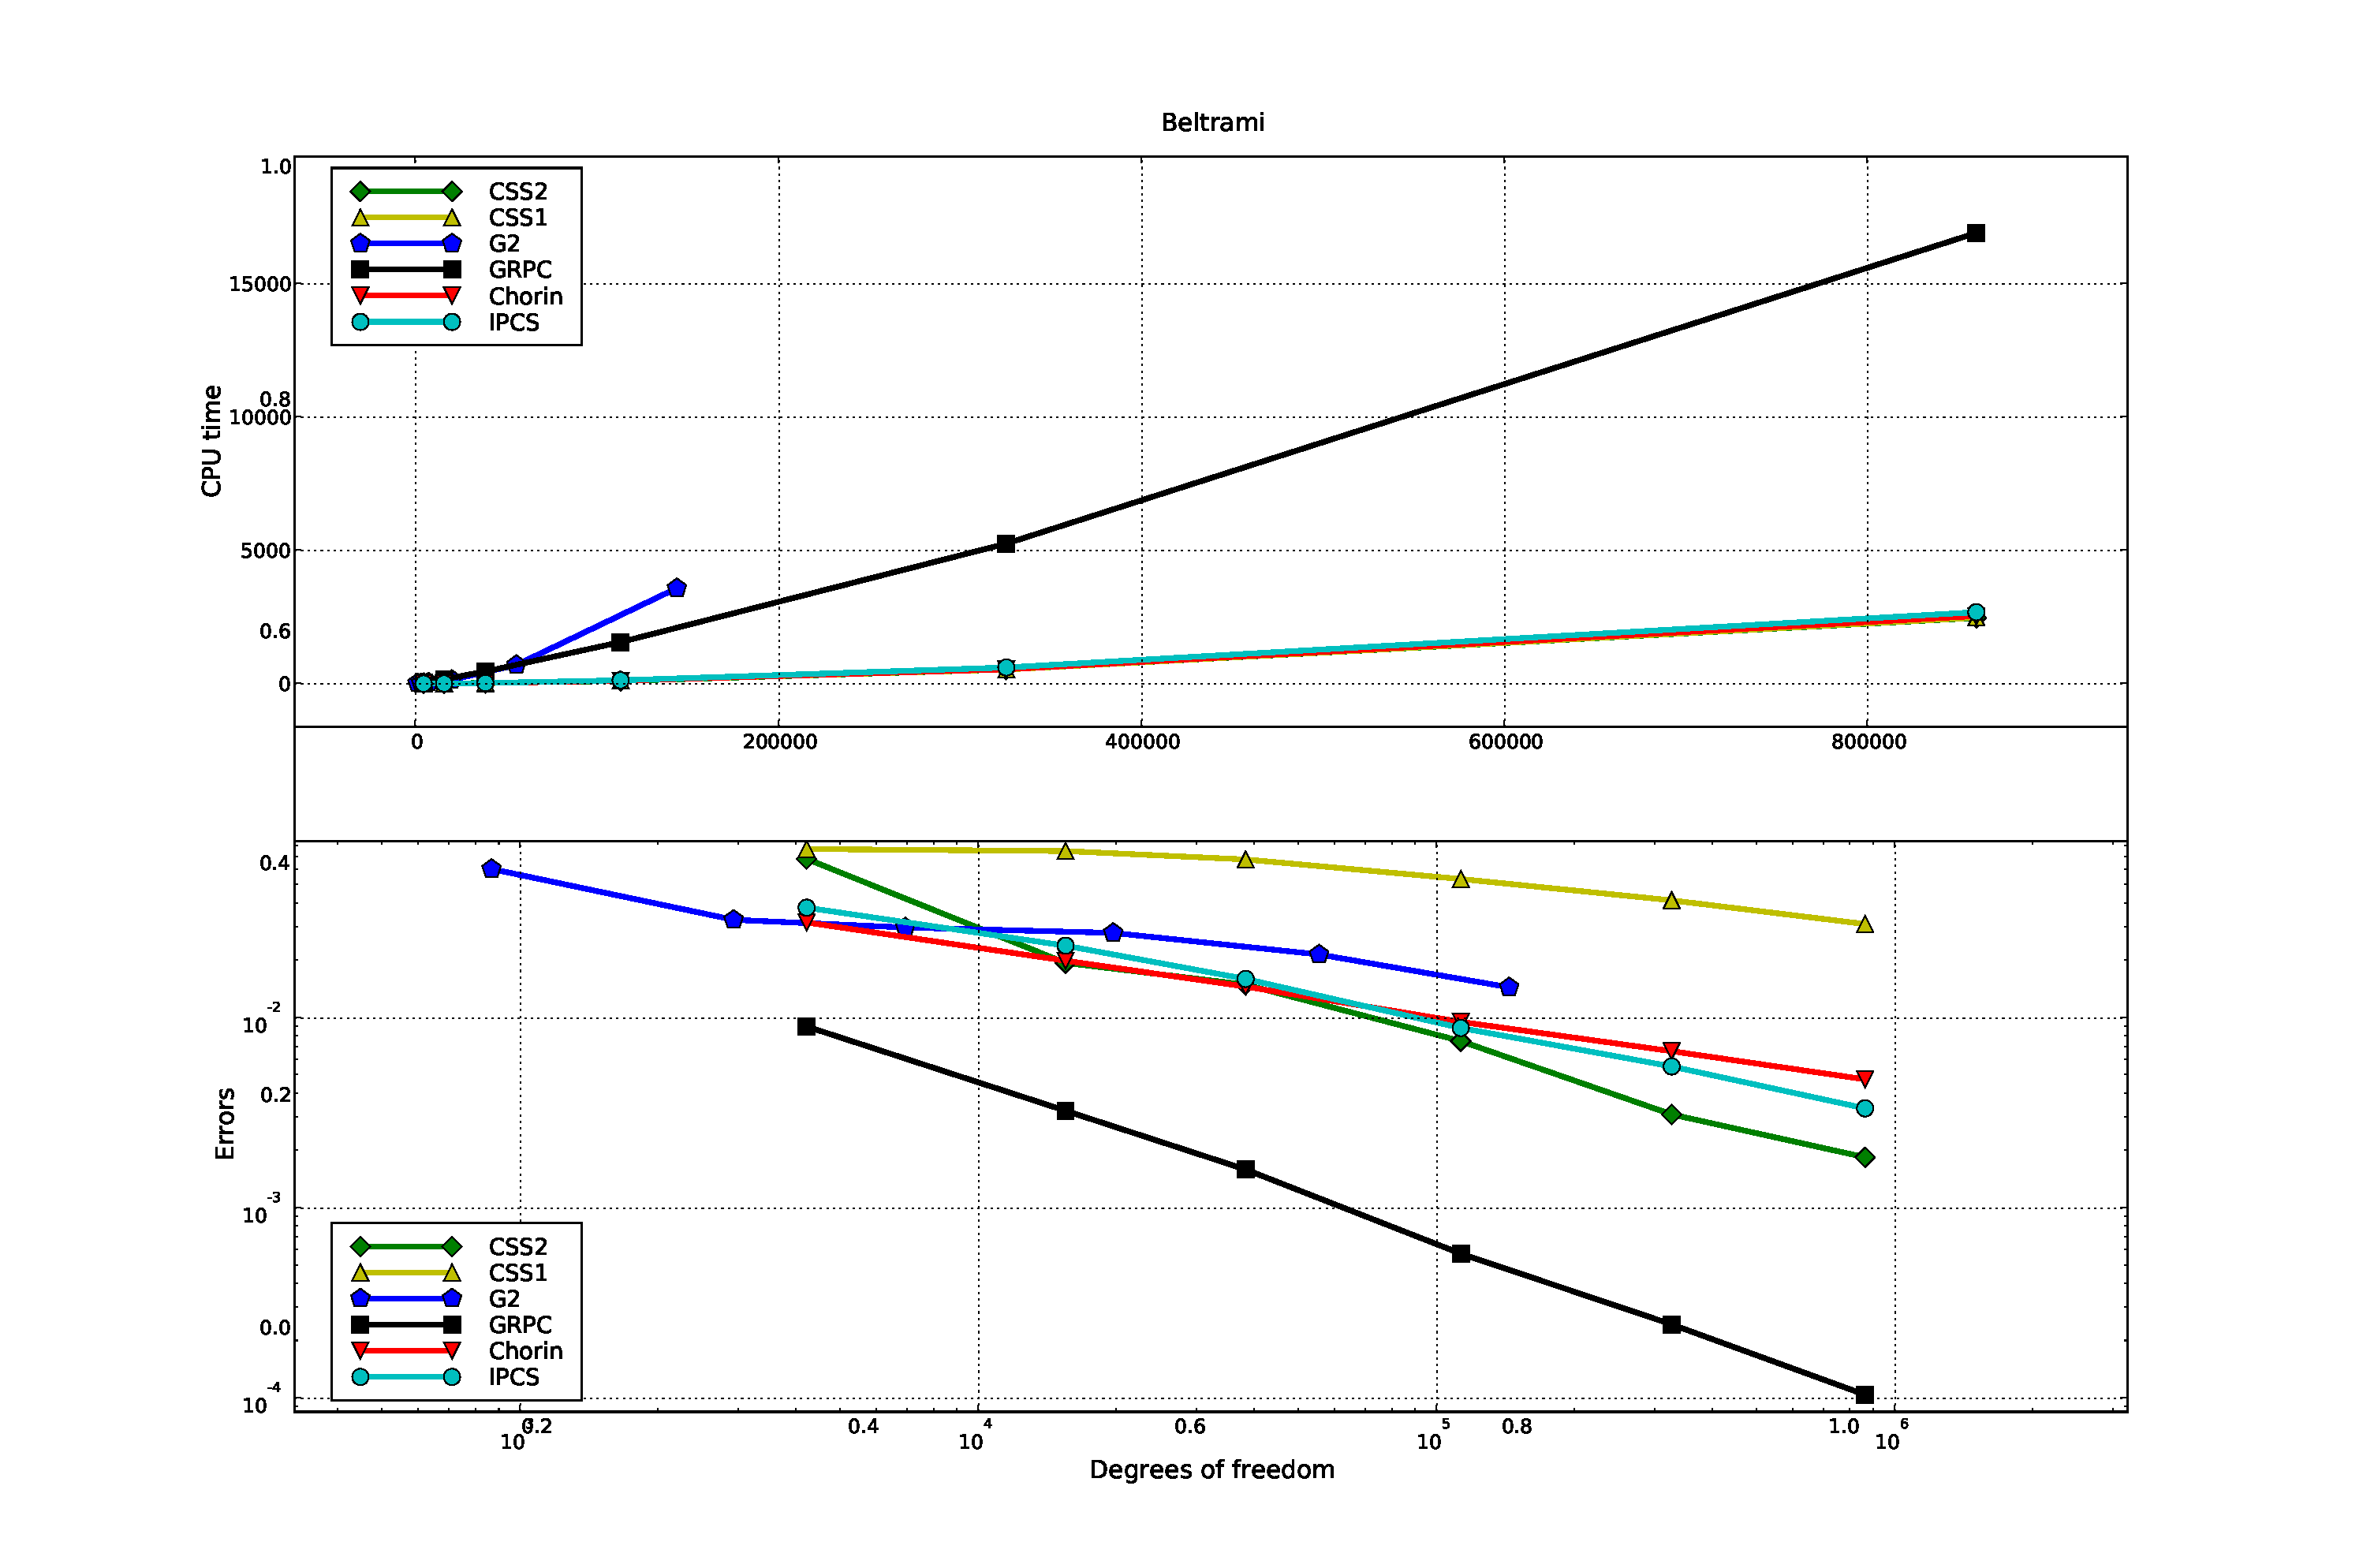
\includegraphics[width=20cm,height=11cm,keepaspectratio=false]{chapters/kvs-1/pdf/new_beltrami_res.pdf}
  \caption{Results for the Beltrami flow test problem.}
  \label{fig:beltrami_res}
\end{figure*}

\subsection{Aneurysm (3D)}

Finally, we consider an idealized geometry modeling an artery with a
saccular aneurysm (see Chapter~\ref{chap:kvs-2}). The diameter of
the artery is set to 4 mm and the length is set to 50 mm. The aneurysm
is of medium size with a radius of 2.5 mm. Inserting the density and
viscosity of blood and suitably scaling to dimensionless quantities,
we obtain a kinematic viscosity of size $\nu = 3.5 / (1.025 \cdot
10^3) \approx 3.4146 \cdot 10^{-6}$. The geometry and flow at the
final time $T = 0.05$ (ms) is shown in Figure~\ref{fig:aneurysm}. We
impose no-slip boundary conditions on the vessel walls. At the inlet,
we set the velocity to $u(x, y, z, t) = \sin(30 t) \, (1 - (y^2 + x^2)
/ r^2)$ where $r = 0.002$ (mm). At the outlet, we enforce a zero
Dirichlet boundary condition for the pressure. As a functional of
interest, we consider the $x$-component of the velocity at a point
$(x, y, z) = (0.025, -0.006, 0)$ (mm) located inside the aneurysm at
final time $T = 0.05$ (ms). A reference value $-0.0355$ (mm/ms) for
this functional was obtained using the IPCS solver on a fine mesh.

\begin{figure}
  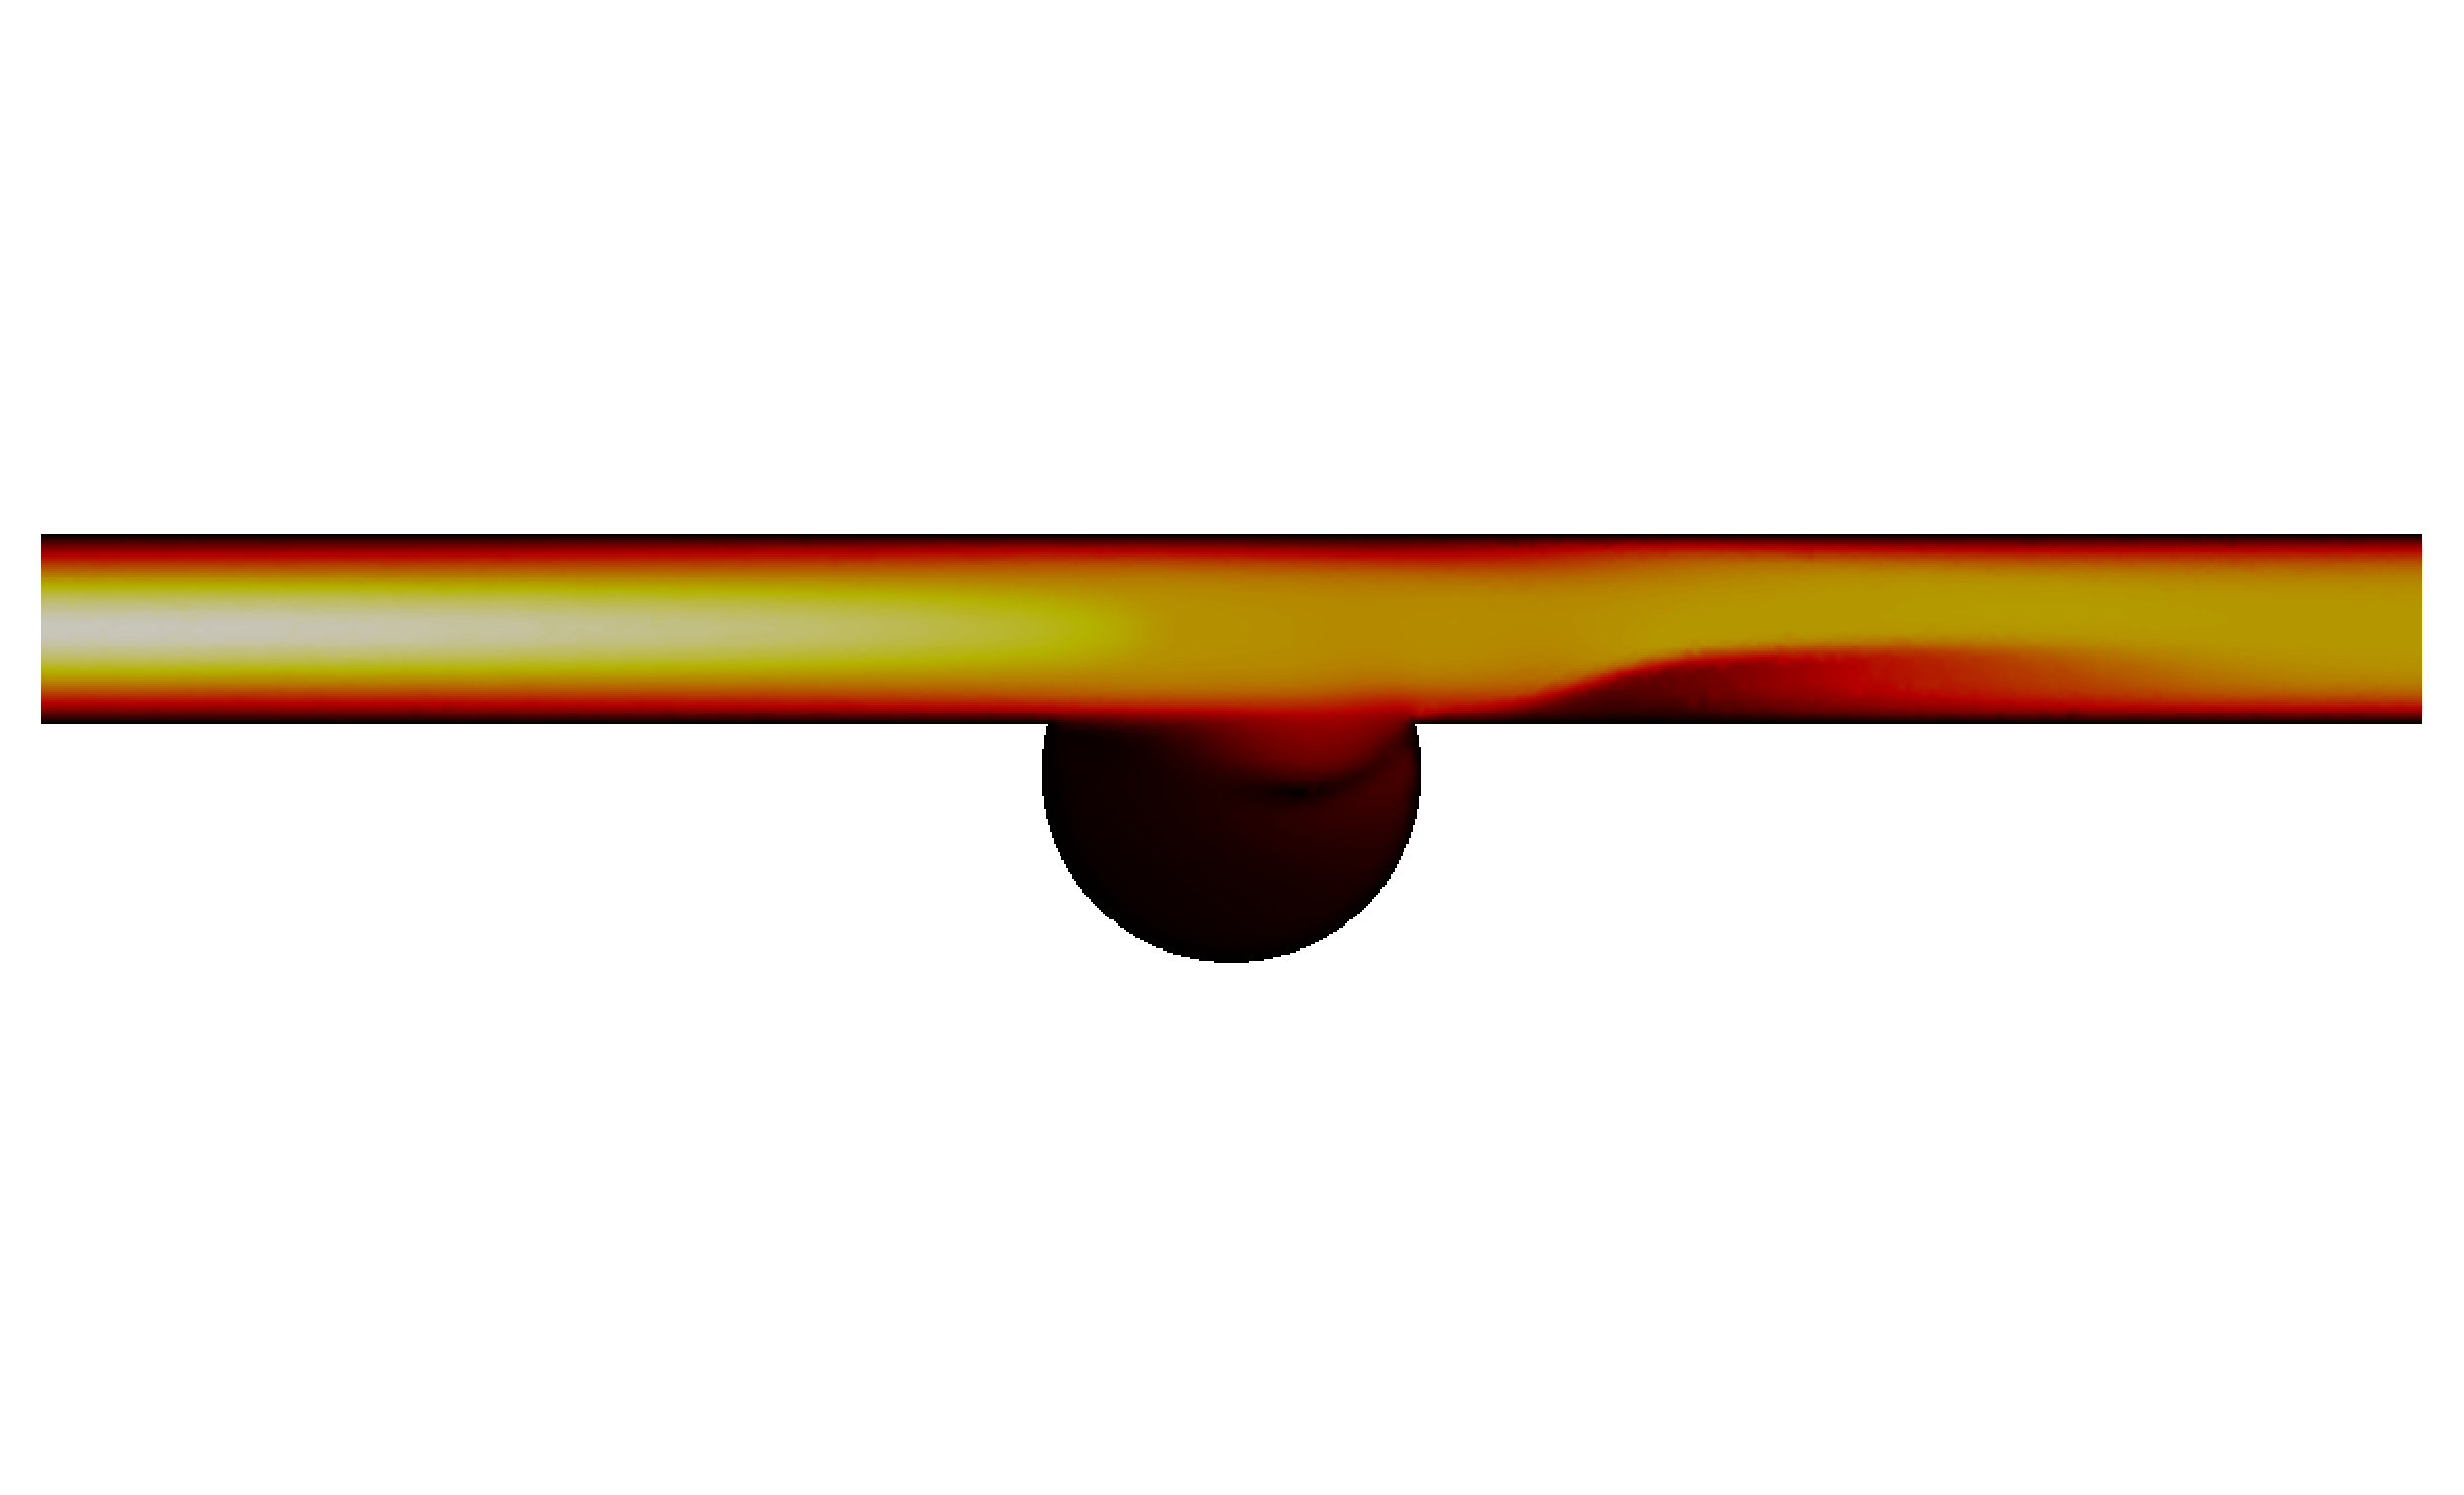
\includegraphics[width=\largefig]{chapters/kvs-1/pdf/aneurysm_at_end_css1.pdf}
  \caption{Velocity magnitude for the aneurysm test problem sliced at
  the center at final time $T = 0.05$ ms.}
  \label{fig:aneurysm}
\end{figure}

\begin{figure*}
  \hspace{-2cm}
  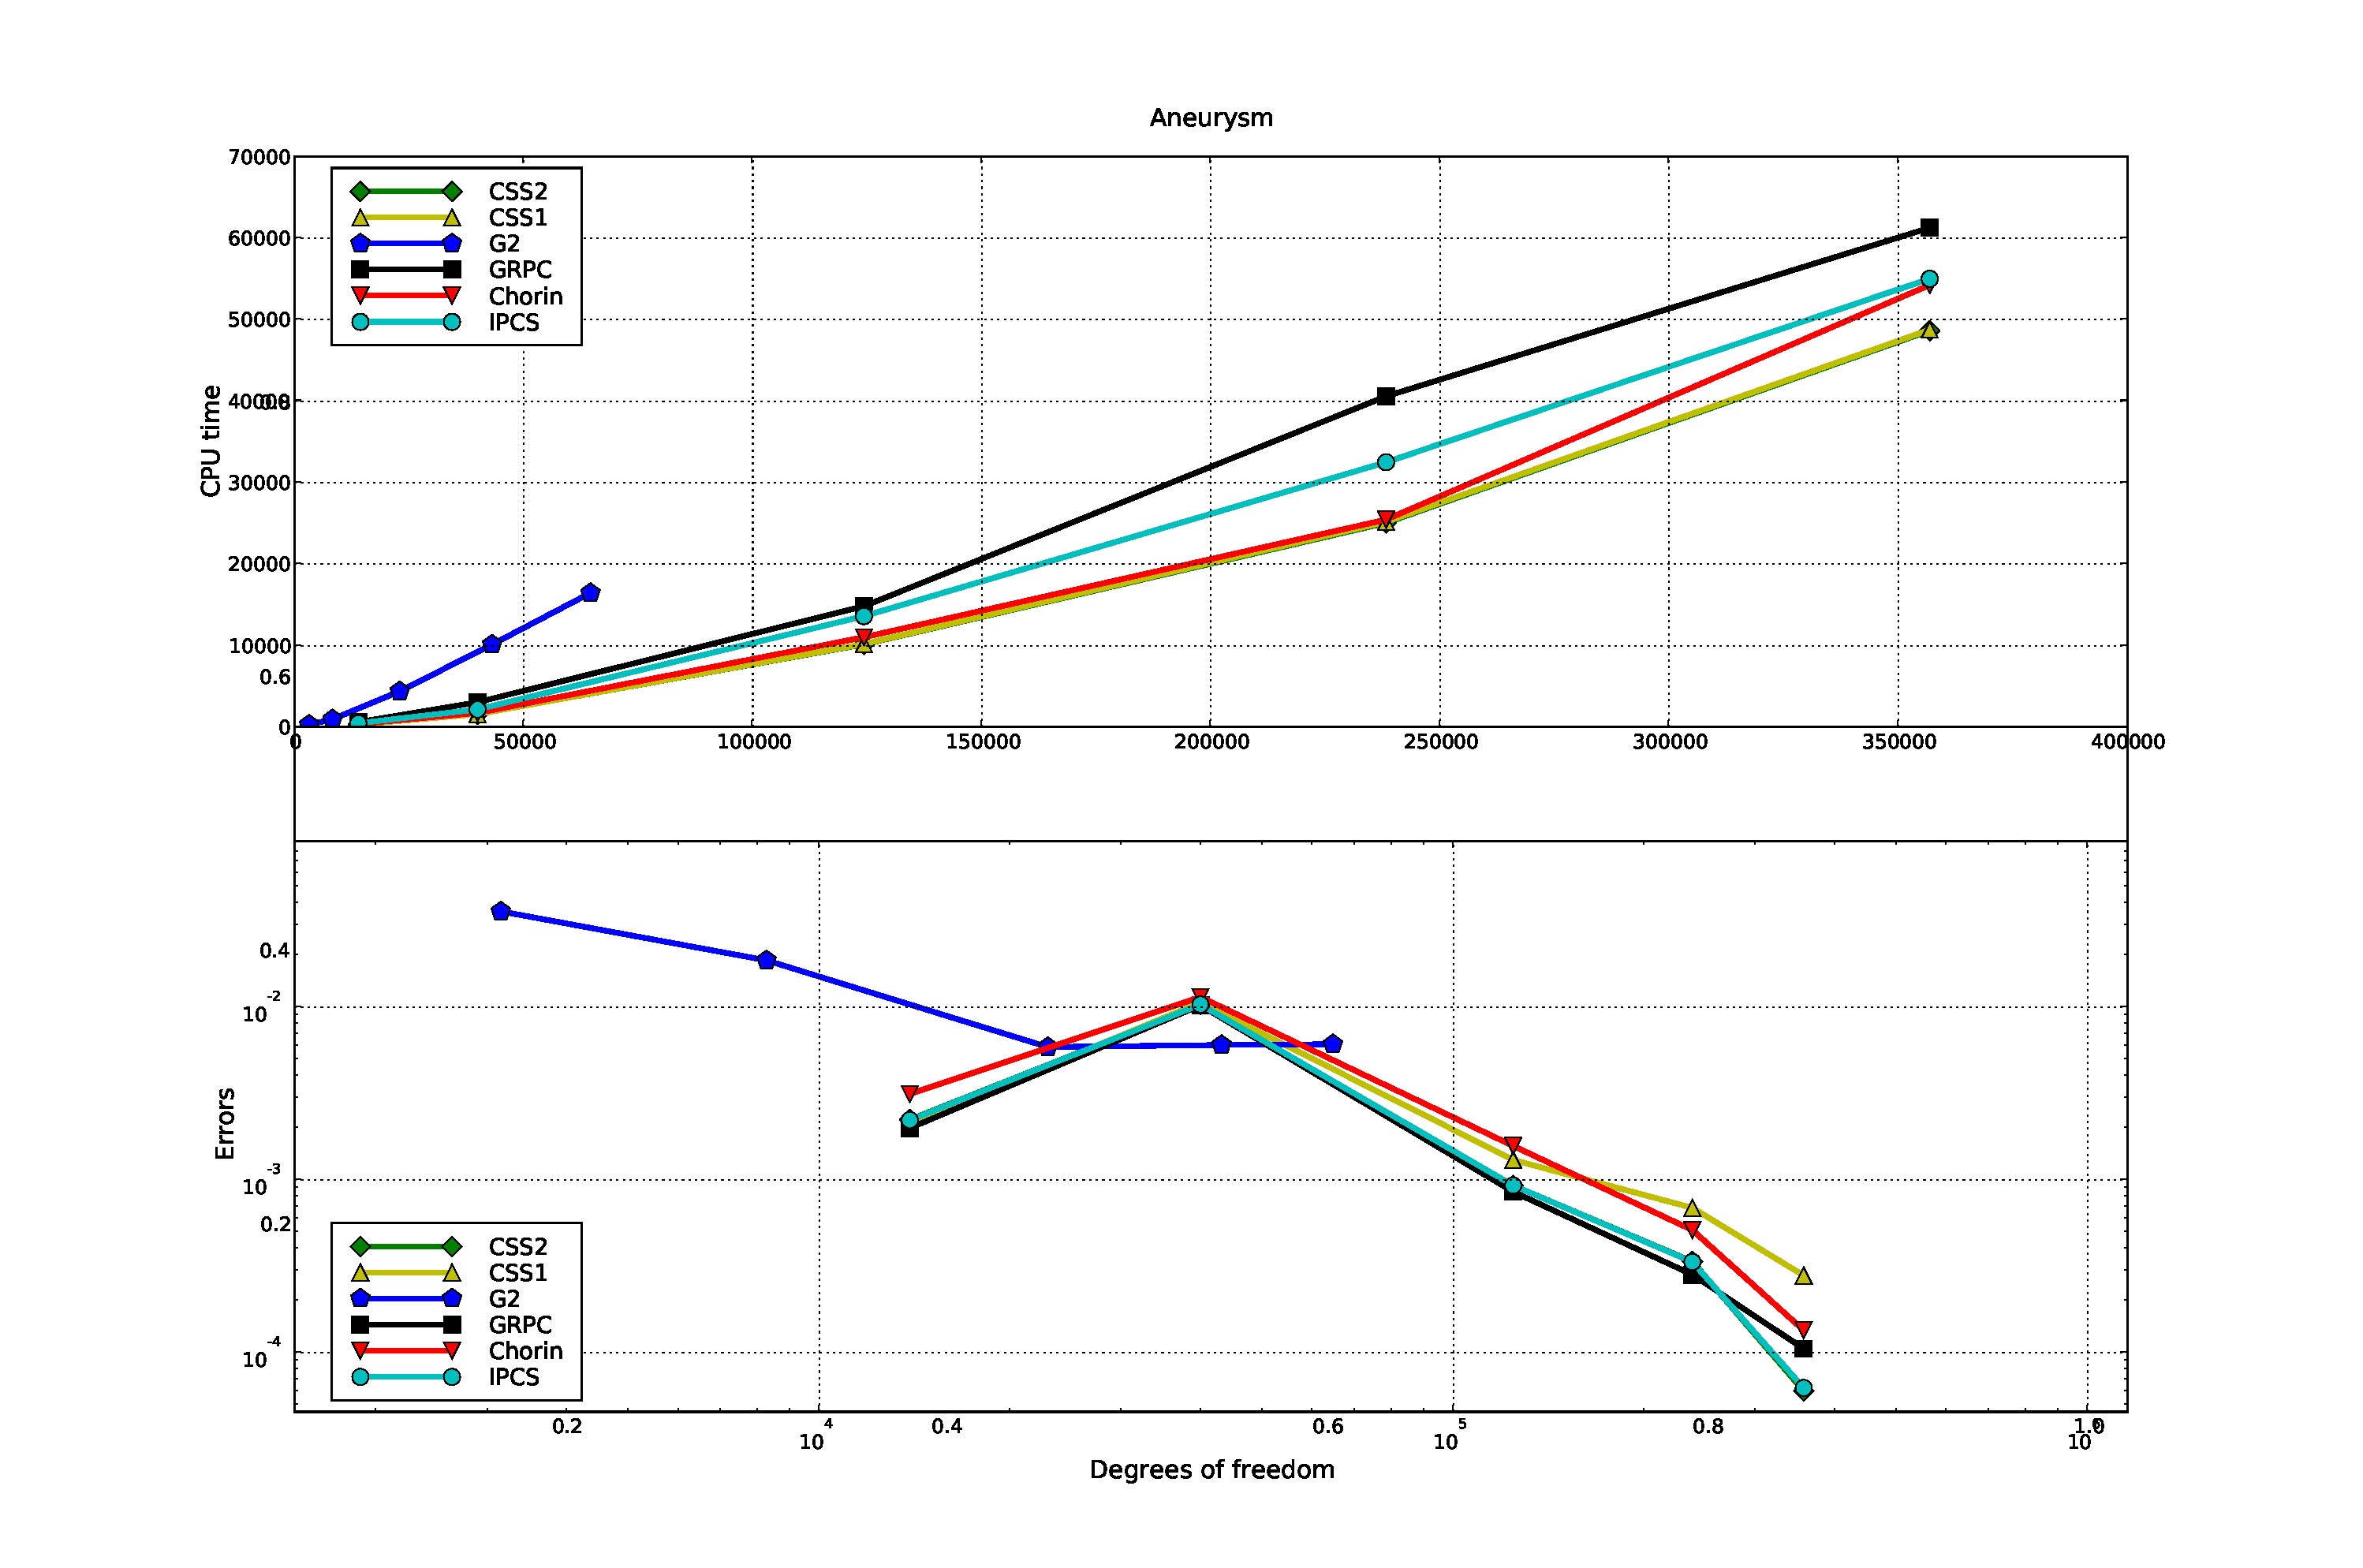
\includegraphics[width=20cm,height=11cm,keepaspectratio=false]{chapters/kvs-1/pdf/new_aneurysm_res.pdf}
  \caption{Results for the aneurysm test problem.}
  \label{fig:aneurysm_res}
\end{figure*}

\paragraph{Results.}

Figure~\ref{fig:aneurysm_res} shows the results for the aneurysm test
problem. Reasonable convergence is obtained for all solvers except the
G2 solver which does not seem to converge towards the computed
reference value.

%------------------------------------------------------------------------------
\section{Summary of results}

To summarize the results for all solvers and test problems, we plot
all timings and errors in a single scatter plot. The rationale behind
the plot is to get an indication of which solver(s) is most accurate
and efficient. Each data point in the plot is the result of solving
one of the above test problems using one particular solver on one
particular refinement level. To be able to compare different test
problems (which vary in simulation time and size of error), the CPU
time is scaled by the average CPU time for all solvers on each
refinement level and the errors are scaled similarly. We also scale
CPU times and errors by the number of degrees of freedom (total number
of unknowns for both velocity and pressure). The resulting scatter
plot is shown in Figure~\ref{fig:scatter}. An ideal solver (which is
both fast and accurate) should be located in the lower left corner of
this plot.

\begin{figure}
  \vspace{0.3cm}
  \hspace{-2cm}
  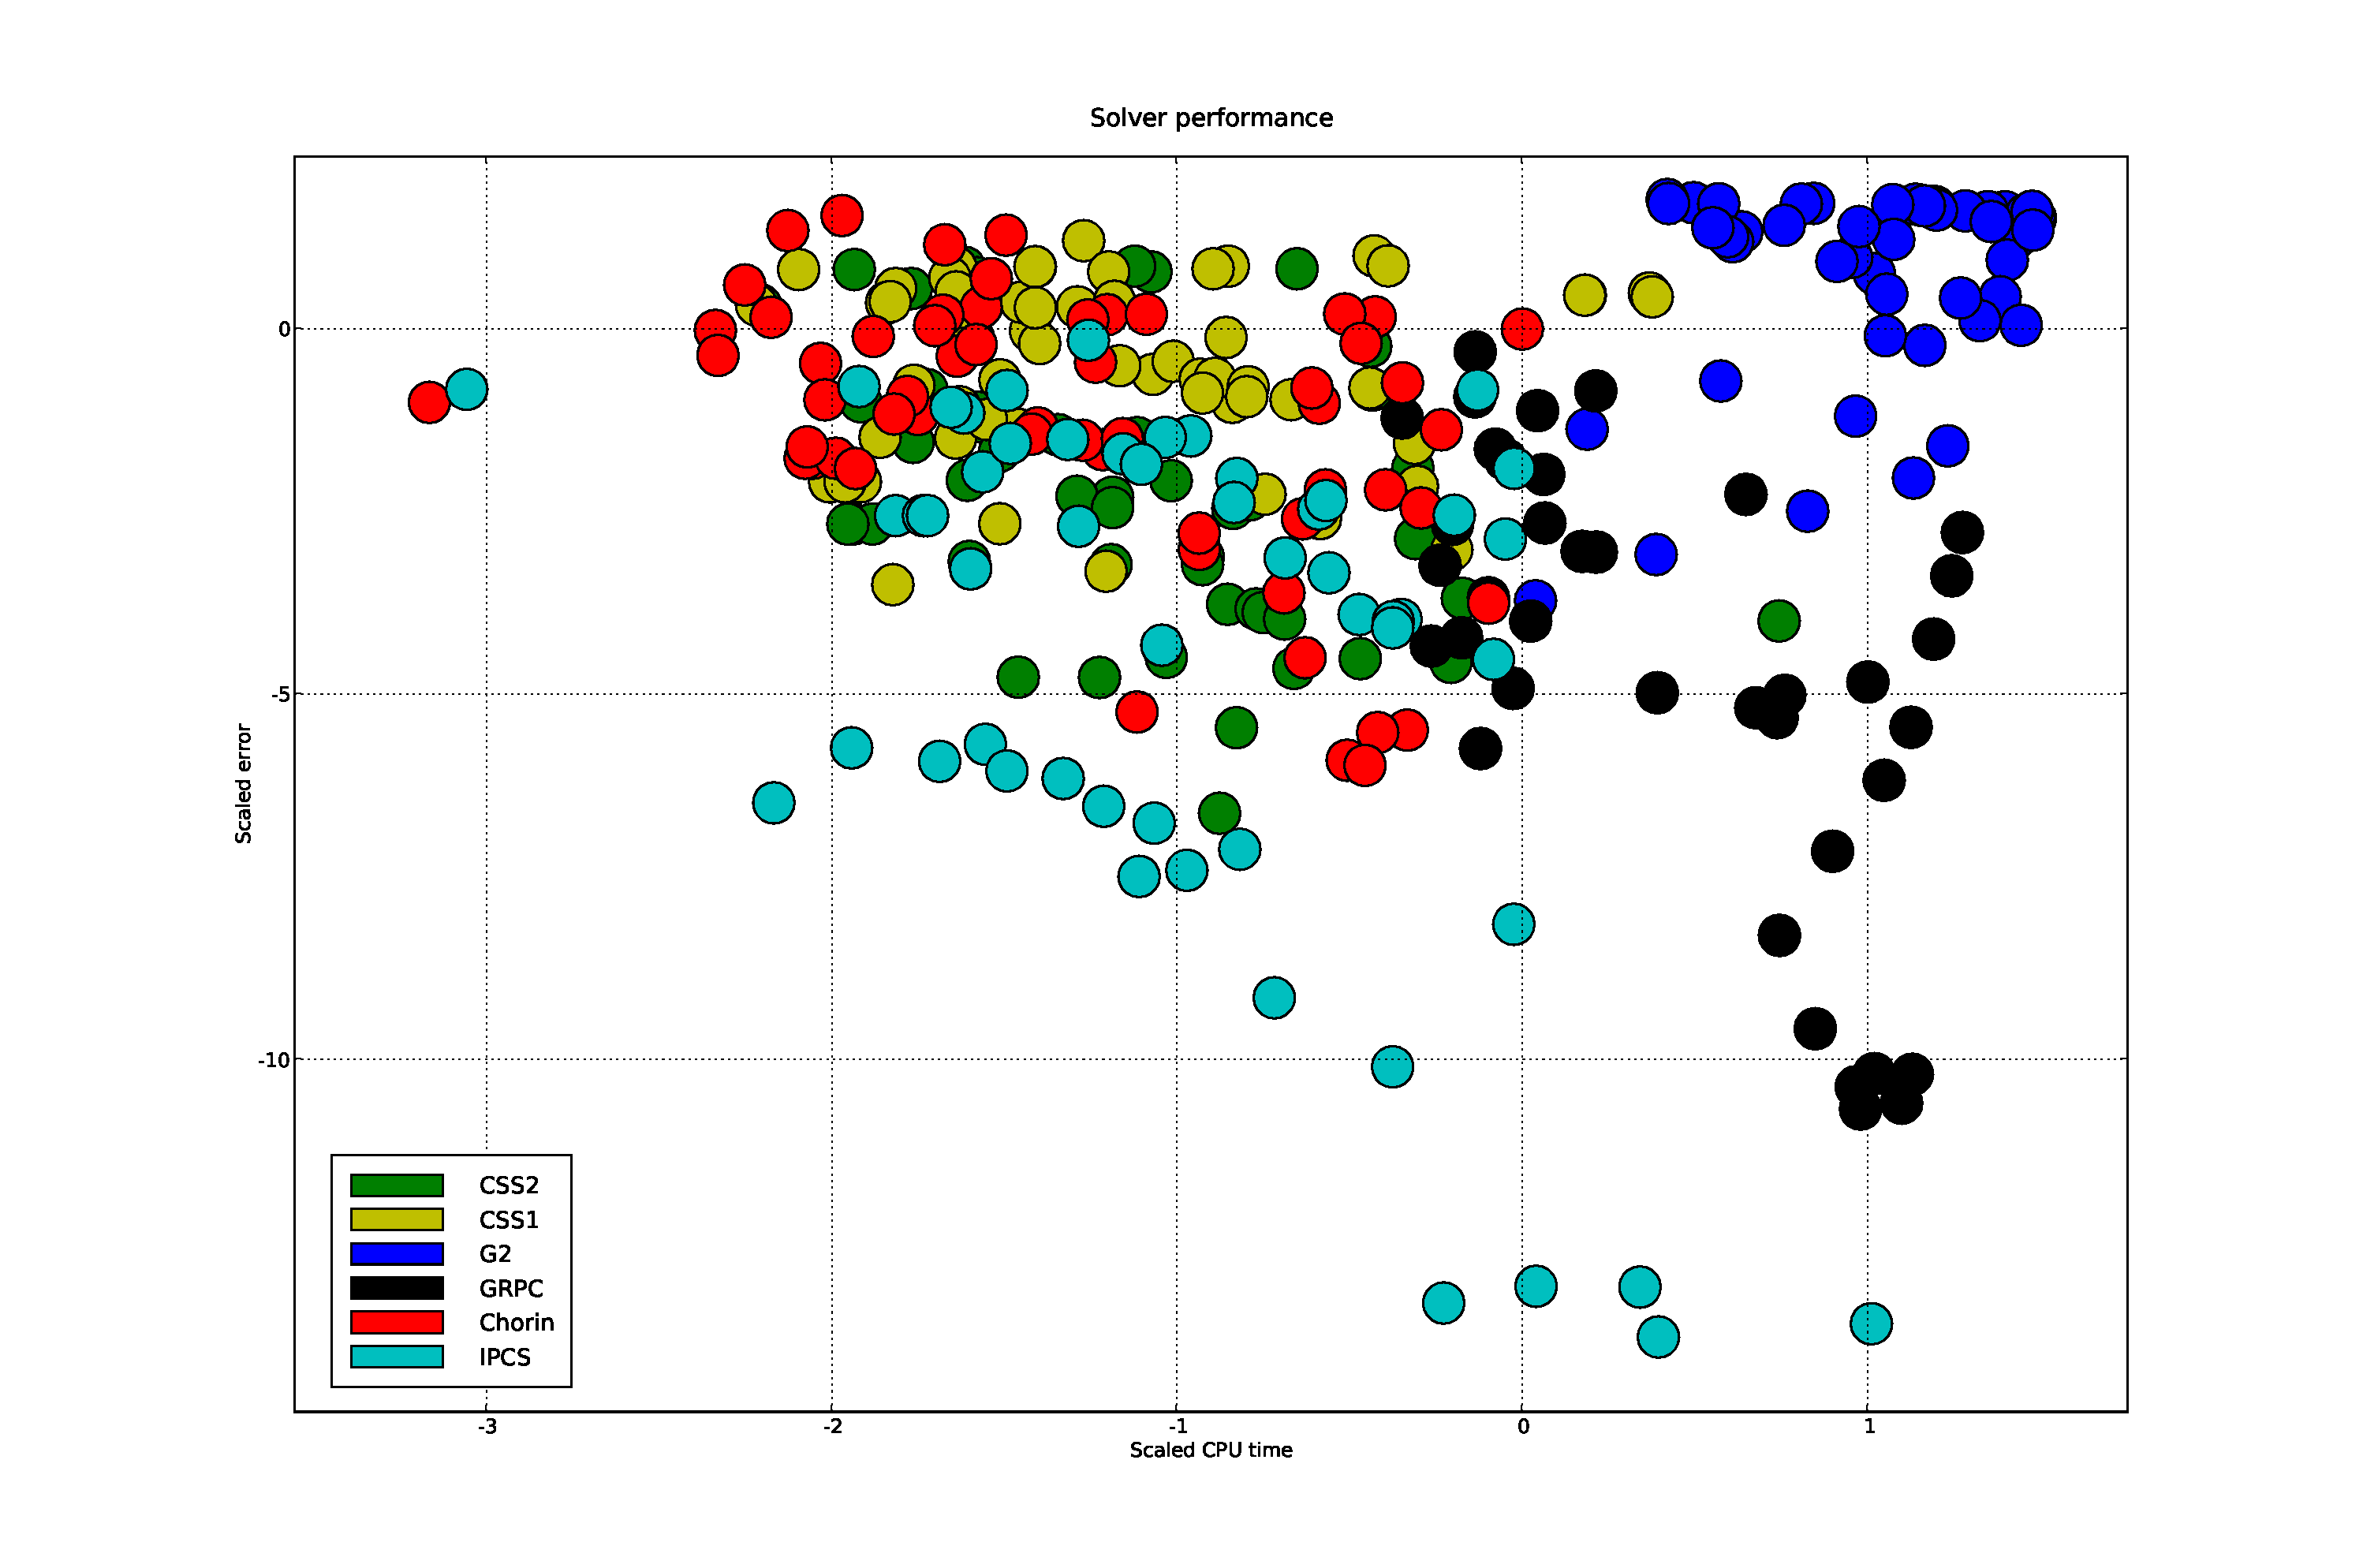
\includegraphics[width=20cm,height=10.5cm,keepaspectratio=false]{chapters/kvs-1/pdf/new_scatter.pdf}
  \caption{Scatter plot summarizing the results for all test problems
    and solvers (logarithmic scale).}
  \label{fig:scatter}
\end{figure}

As can be seen in Figure~\ref{fig:scatter}, the Chorin, \css{1} and
\css{2} solvers have an average performance and are mostly clustered
around the center of mass of the scatter plot. The G2 solver is mainly
located in the upper right corner. The results for the IPCS solver are
less clustered but it is the solver with most points located in the
lower left corner. The GRPC solver is mostly located in the lower
right corner of the scatter plot, indicating that it is accurate but
expensive.

%------------------------------------------------------------------------------
\section{Discussion}
\label{Discussion}

\subsection{Numerical boundary layers}

As pointed out in \citet{GuermondMinevShen2006}, the fractional step
solvers are usually plagued by an artificial boundary layer, because
the boundary condition $ \nabla p^n_h \cdot n |_{\partial\Omega}=0$ is
enforced on the pressure. This 'unphysical' Neumann boundary condition
can create a numerical boundary layer simply because the velocity
update $u^{n}_h=u^{n-1}-\deltat\nabla p^n_h$ may lead to non-zero
velocities in the tangential direction on no-slip walls (this follows
since there is nothing preventing the pressure gradient from being
non-zero in the tangential direction). However, in this work the
velocity is being updated through a weak form where the no-slip
boundary condition is strongly enforced. As such, the tangential
velocity is set to zero and an artificial boundary layer is not
observed in our simulations using the fractional step solvers Chorin
and IPCS.

\subsection{Time discretization}

For the channel test problem, the convective term is zero and the
discretization of the diffusive term is of particular importance. A
formally second-order accurate in time Crank--Nicolson type scheme for
the viscous term will in general improve the accuracy over the merely
first-order explicit or fully implicit schemes. This is why the GRPC,
IPCS and G2 solvers perform well on this problem. The channel test
problem is the problem where G2 performs best relative to the other
solvers, which could also be attributed to the fact that both
stabilization terms in the momentum equation of G2 are zero for this
flow.

%------------------------------------------------------------------------------
\section{Conclusions}

From the scatter plot in Figure~\ref{fig:scatter}, we conclude that
the IPCS solver is overall the most efficient and accurate
method. Another advantage of the IPCS method is that it is easy to
implement and does not require the iterative solution of a nonlinear
system in each time step. The GRPC method (straightforward standard
finite element Galerkin discretization) also obtains high accuracy,
but does not deliver the same speed. It is possible that better tuning
of the iterative solution of the saddle-point system would change this
picture.
